\pdfoutput=1
\documentclass{JINST}
\usepackage{caption}
\usepackage{subcaption}
\title{Double Chooz Physical Environment Monitoring System}

\author{Pi-Jung Chang$^a$, Glenn Horton-Smith$^a$\thanks{Corresponding
author.}~ , David McKee$^a$, Deepak Shrestha$^a$, Lindley Winslow$^b$, and Janet Conrad$^b$ \\
\llap{$^a$}Department of Physics, Kansas State University,\\
  Cardwell 116, Manhattan, KS 66506, USA\\
\llap{$^b$}Department of Physics, Massachusetts Institute of Technology,\\
  77 Massachusetts Avenue, Bldg. 26-537 Cambridge, MA 02139, USA\\
  E-mail: \email{gahs@phys.ksu.edu}}
\abstract{ The Double Chooz experiment will measure reactor antineutrino flux from two detectors with a relative normalization uncertainty less than 0.6\%. The Double Chooz physical environment monitoring system records conditions of the experiment's environment to ensure the stability of the active volume and readout electronics. The system monitors temperatures in the detector liquids, temperatures and voltages in electronics, experimental hall environmental conditions, magnetic field, radon concentrations in the air, and phototube high voltages. The system scans all channels automatically, stores data in a common database, and warns of changes in the detector's physical environment. The total isotope radioactivity of all sensor assemblies in the liquid detector is estimated by three dimensional distribution in the detector and is smaller than the background rate which should be considered in the final Double Chooz result. The design, performance and the radioactivity of the Double Chooz physical environment monitoring system will be presented in this article.}


\keywords{Double Chooz; environment monitoring system; radioactivity}

\begin{document}

\section{Introduction}
 The purpose of the Double Chooz experiment is searching for a non-vanishing mixing angle $\theta_{13}$ with two identical liquid detectors.
The Double Chooz detector system is a four-layer concentric cylindrical detector with a calibration system. The innermost acrylic vessel is filled with the 10.3 m$^{3}$ $\nu$-target liquid. The $\nu$-target liquid (NT) is consisted of n-dodecane, 2,5-diphenyloxazole, bis-(2-methylstyryl)benzene, ortho-phenylxylylethane, and 1 g gadolinium/l.~\cite{bib1}  The NT is surrounded by the gamma catcher (GC) which is a 55 cm thick liquid scintillator layer without Gd.~\cite{bib2}~\cite{bib1a} The NT and GC are in 8 mm and 12 mm thick acrylic vessels.
The third layer is the buffer, which is filled with 105 cm thick mineral oil. The fourth layer is the inner veto tank, a 50 cm thick liquid scintillator.~\cite{bib1}  The main cylindrical detector is coved by an outer veto system, a plastic scintillator assembly.~\cite{bib2}~\cite{bib1a}



%The detector system is consisted of a series of cylinder vessels, a calibration system and an outer veto. The most inner vessel is called $\nu$-target, a 8 mm thick acrylic vessel, filled with liquid scintillator loaded with 1 g gadolinium/l and is surrounded by a $\gamma$-catcher, a 55 cm thick nonloaded liquid scintillator with the same optics property.\cite{bib1} Outside the $\gamma$-catcher vessel is a 105 cm thick buffer region filled with non scintillating oil which serves to decrease the level of accidental background. \cite{bib1,bib2} An inner veto vessel is the most outside region of the cylinder system and it is a 50 cm thick liquid scintillator layer.\cite{bib1}

The Double Chooz physical environment monitoring system records conditions of the experiment's environment which can impact the experiment\textquoteright s goals. The monitoring system includes liquid temperatures, magnetic fields of PMTs, radon concentrations, the humidity of the laboratory and photo-tube high voltages. This system scans all channels automatically, stores data in a common database and warns shifters unusual situations\cite{bib3}

Most function in this system can be accomplished by 1-Wire$\circledR$ Dallas Semiconductor.\cite{bib4} We can use a single master bus for multi-function controls and operations supporting multiple devices on a single line. A server could be a 10 inch laptop to run the master bus and read a certain time period by a program written in C++. Every device has a unique unalterable factory-laser ID which can be identified easily. The data can be accessed by an online data acquisition system from the database and the control system which can give a feedback to shifters.\cite{bib3} Figure ~\ref{fig1} is a physical environment monitoring system schematic cartoon.
\begin{figure}
\centering
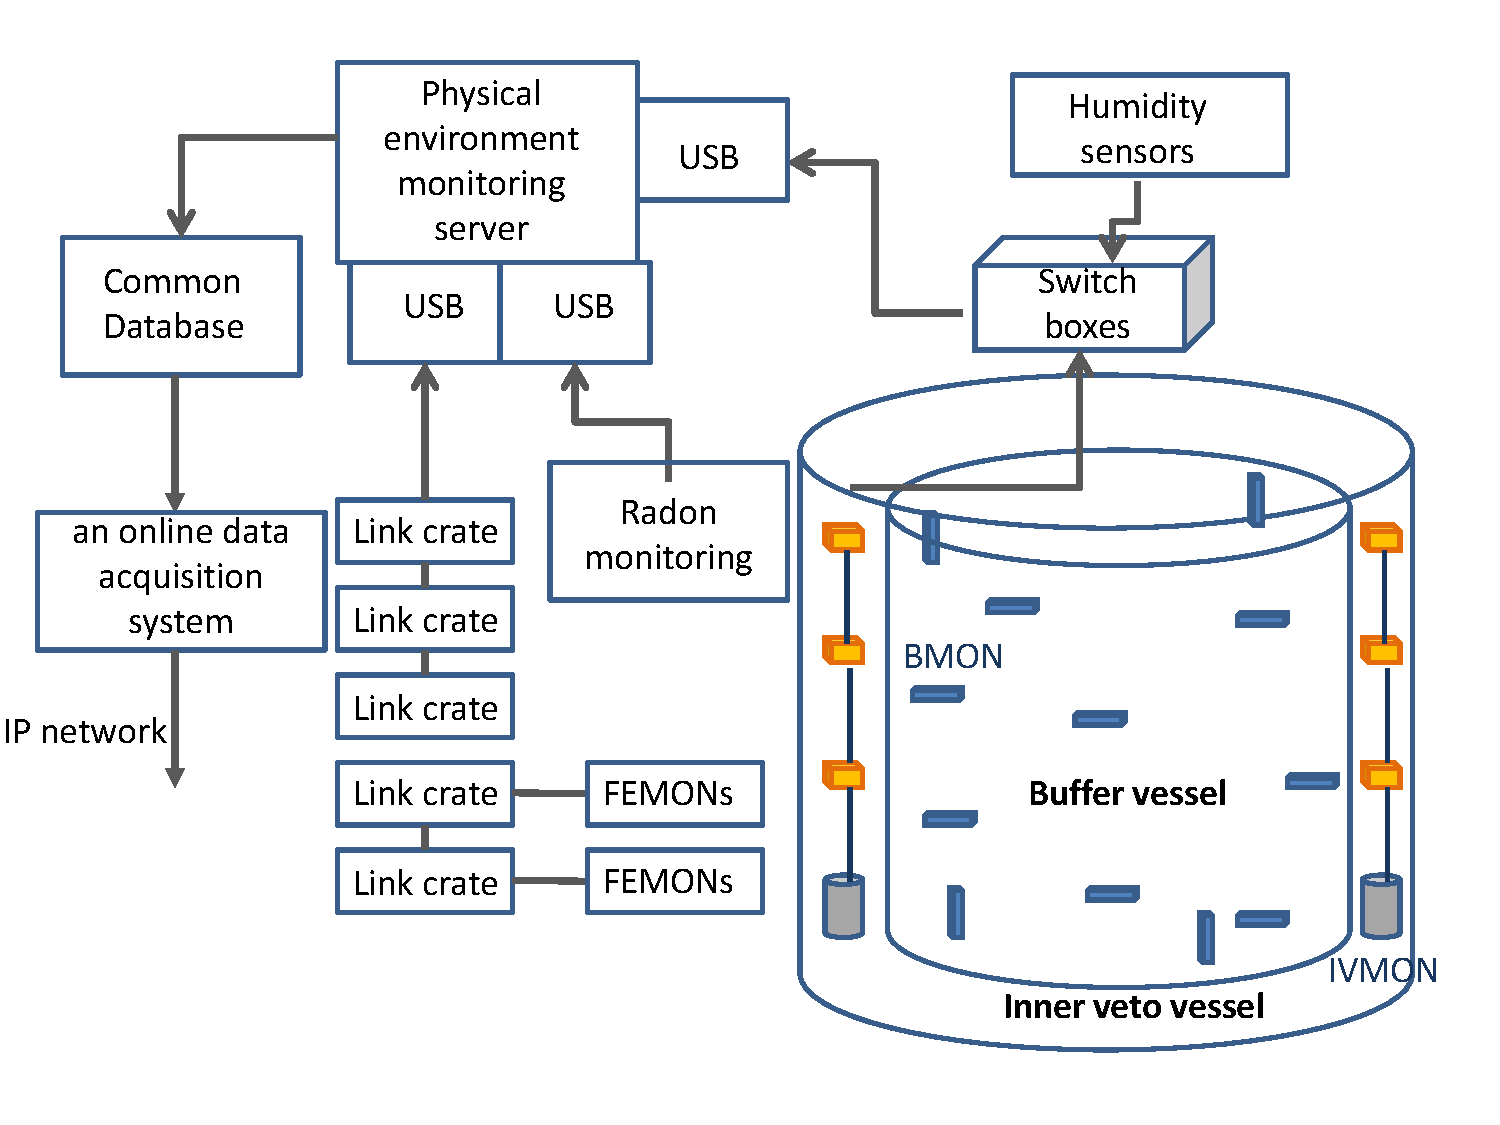
\includegraphics[width=.6\textwidth]{slowmonpic.pdf}
\caption{Physical environment monitoring system schematic cartoon.}
\label{fig1}
\end{figure}

\section{Sensors read by 1-Wire devices }
The sensors with 1-Wire devices are connected the bus with a high-speed 12Mbps Universal Serial Bus(USB) interface, DS9490.\cite{bib5} A single wire is sufficient for operating and functioning all devices on a loop; however, we still support 5V to IC power supply pins in order to reduce a current burden of the server. Each sensor assembly needs a standard "RJ11" 6P6C modular connector to hook on a switch box. Each switch box has 6 branches of RJ11 sockets providing 5V for IC power supply pins of 1-Wire chips and 12V for Buffer vessel monitors (BMONs). Six branches are from three MicroLAN couplers\cite{bib6}, DS2409. Each DS2409 can prove two branches, main and auxiliary 1-Wire outputs, and be programmed to open drains and control outputs by the master bus.(see Figure ~\ref{fig2}.) A communication speed of DS2409 is 16.3k bits per second. In order to avoid static damages , we put one ESD protection diode on 1-Wire outputs of DS2409.

\begin{figure}[h]
\centering
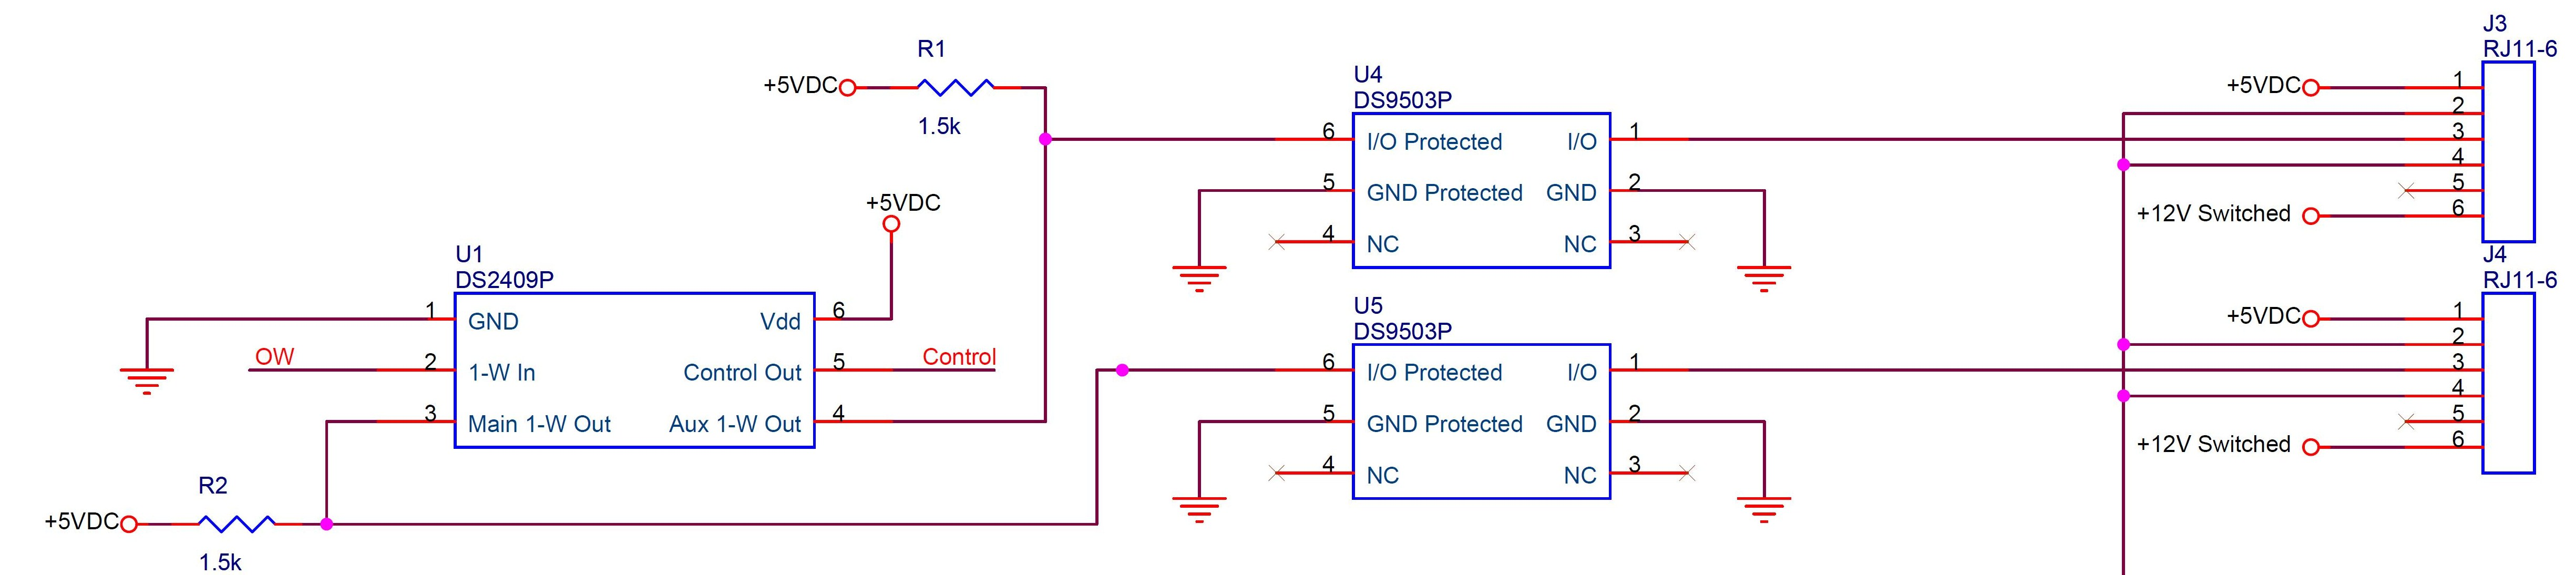
\includegraphics[width=.6\textwidth]{switchbox.jpg}
\caption{Schematic layout of partial switch box.}
\label{fig2}
\end{figure}
\subsection{Sensors are sunk in the liquid}
Main sensors can be divided two types. The first typical sensors are sunk into the liquid. Two kinds of monitors are used, BMON and Inner veto vessel monitor (IVMON).In order to be waterproof, they are epoxy-potted on acrylic base plates and put in buffer and inner veto liquids. Each BMON is mounted a three-axis magnetometer, HMC2003,\cite{bib7} and a thermometer. The magnetometer is a three magneto-resistive sensors assembly and operated by a 12 V power supply. Its measurable range is $\pm$ 2 gauss and sensitivity is 40 microgauss. An ADC chip from Dallas Semiconductor accesses the output voltage of 2.5V+B$\ast$(1V/gauss). In order to reach high resolution, the control program sends a 0 or 1 signal to a NPN amplifier which would set/reset a current strap called SR$_{+}$/ and SR$_{-}$ pins. (see Figure ~\ref{fig3}.) A set/reset action can flip the magnetization of the permalloy film in side the magnetometer and also the output voltages.\cite{bib8}

\begin{figure}
\centering
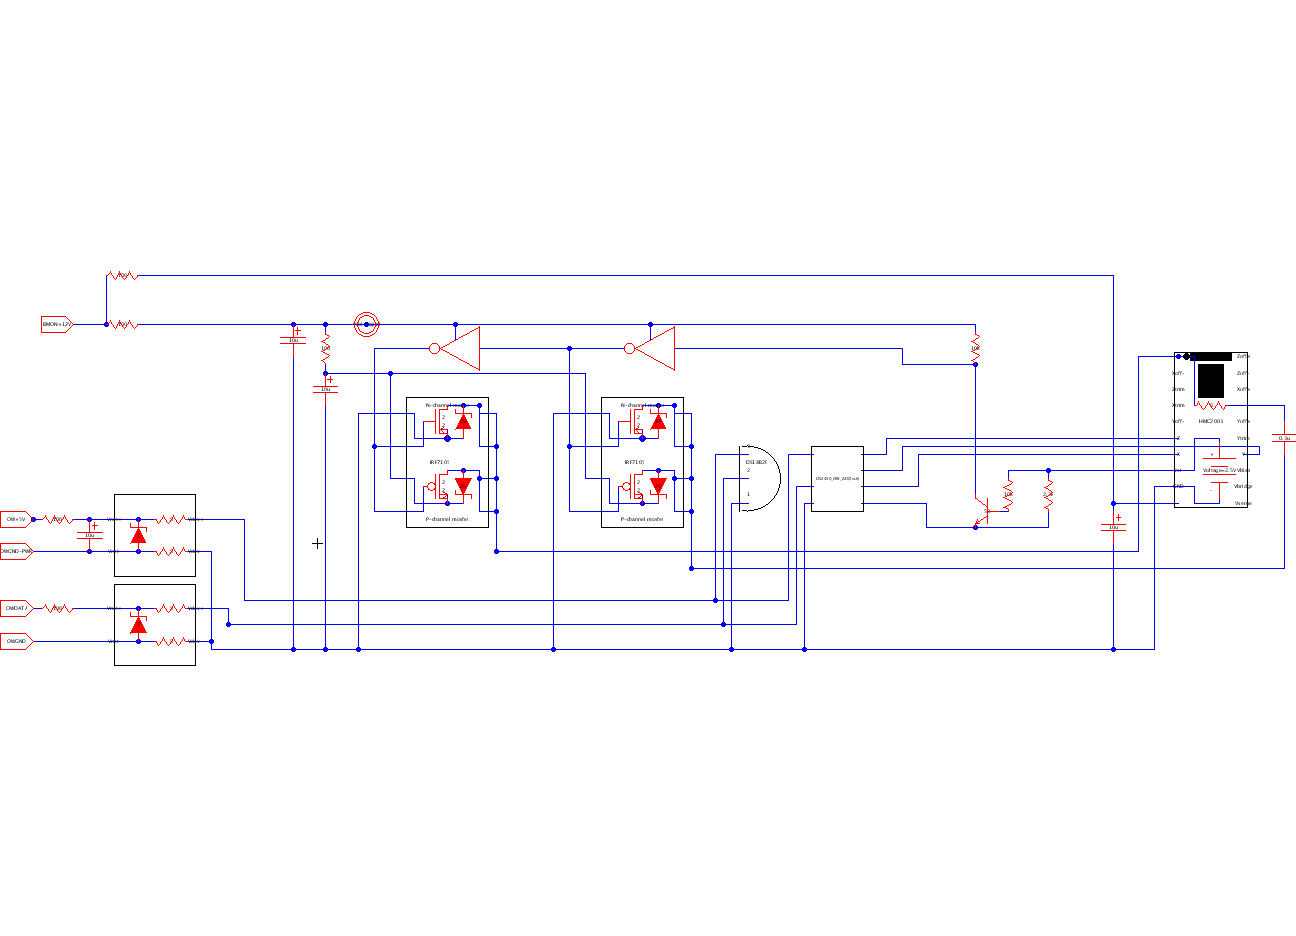
\includegraphics[width=.6\textwidth]{bmon_schematic.png}
\caption{Schematic layout of BMON.}
\label{fig3}
\end{figure}
The thermometer, DS18B20 \cite{bib6}, is a digital thermometer which can operate from -55$^\circ$C to 124$^\circ$C and its accurate is about $\pm$5$^\circ$C. There are 12 BMONs distributed uniformly in the buffer vessel. They will collect data of PMT\textquoteright s magnetic field and liquid temperature in the buffer vessel. There are total 20 IVMONs distributed in the inner veto vessel, on the inner veto vessel lid, on bottom of a liquid expansion tank and a pit pipe. Every four IVMONs will be consisted of a loop string. A BMON and a IVMON prototypes are presented on Figure ~\ref{fig4a} and ~\ref{fig4b}.

\begin{figure}
        \centering
        \begin{subfigure}[b]{0.5\textwidth}
                \centering
                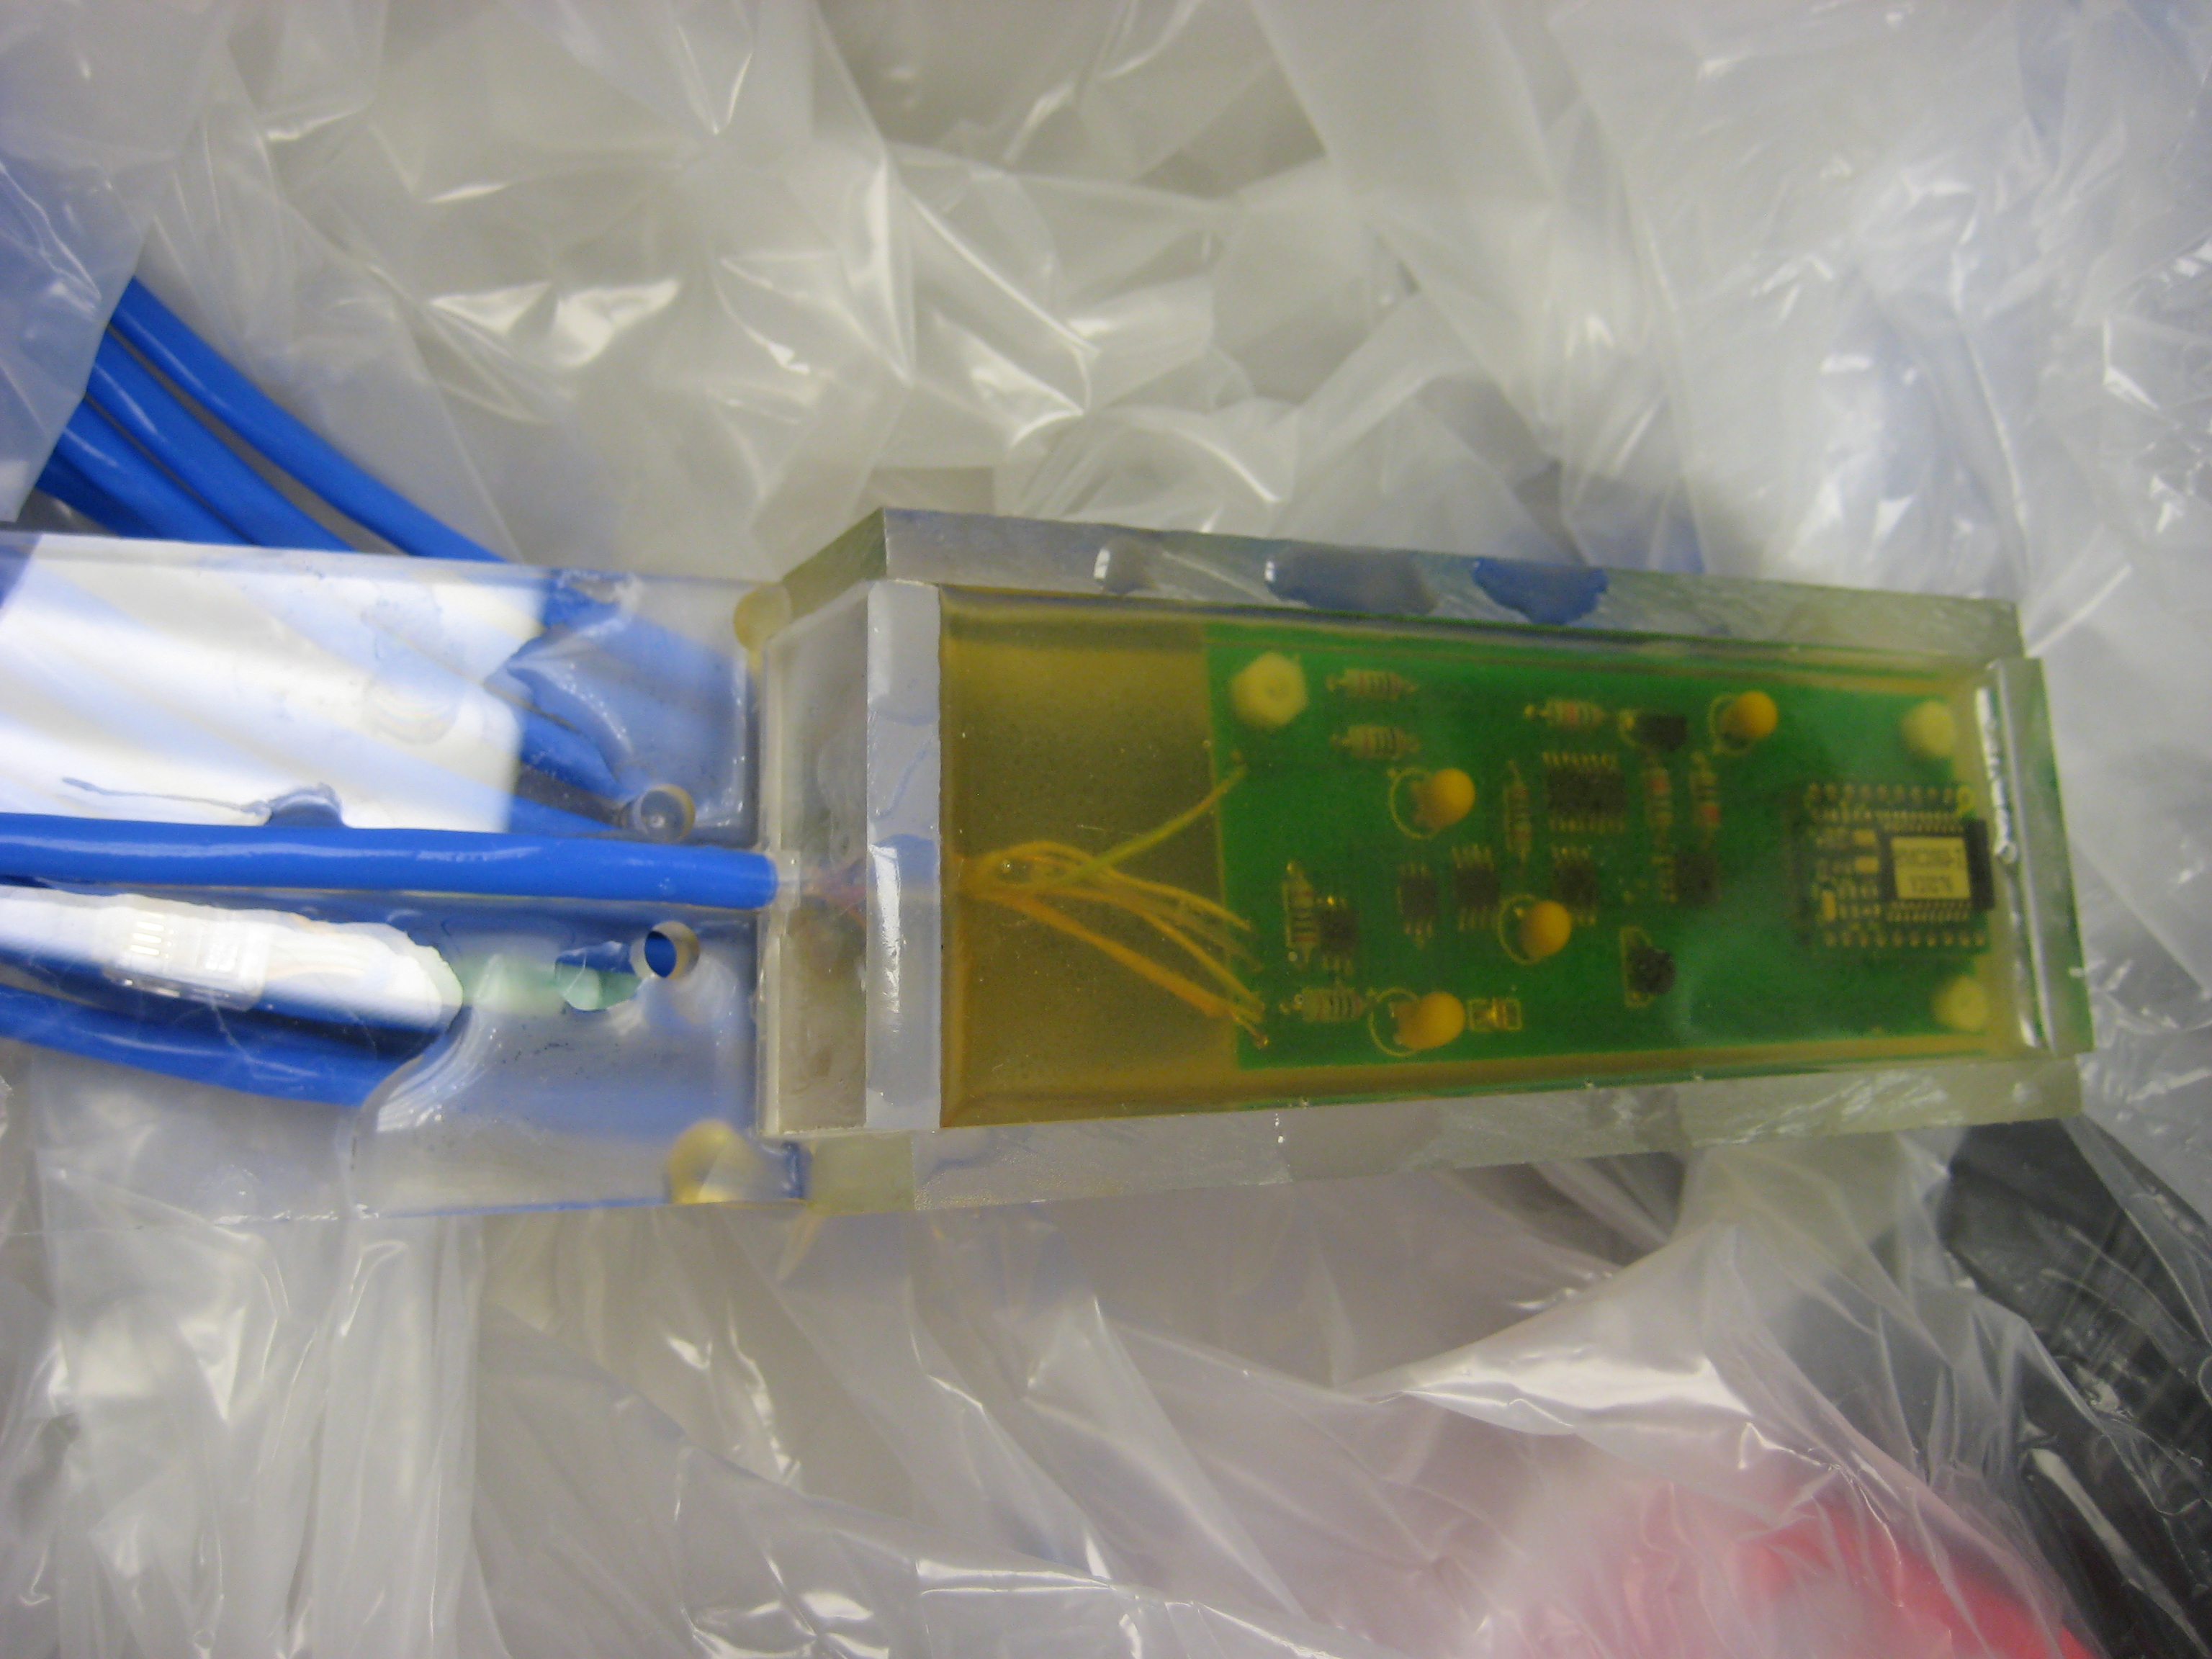
\includegraphics[width=\textwidth]{IMG_2884.JPG}
                \caption{A BMON prototype.}
                \label{fig4a}
        \end{subfigure}%
        ~ %add desired spacing between images, e. g. ~, \quad, \qquad etc.
          %(or a blank line to force the subfigure onto a new line)
        \begin{subfigure}[b]{0.5\textwidth}
                \centering
                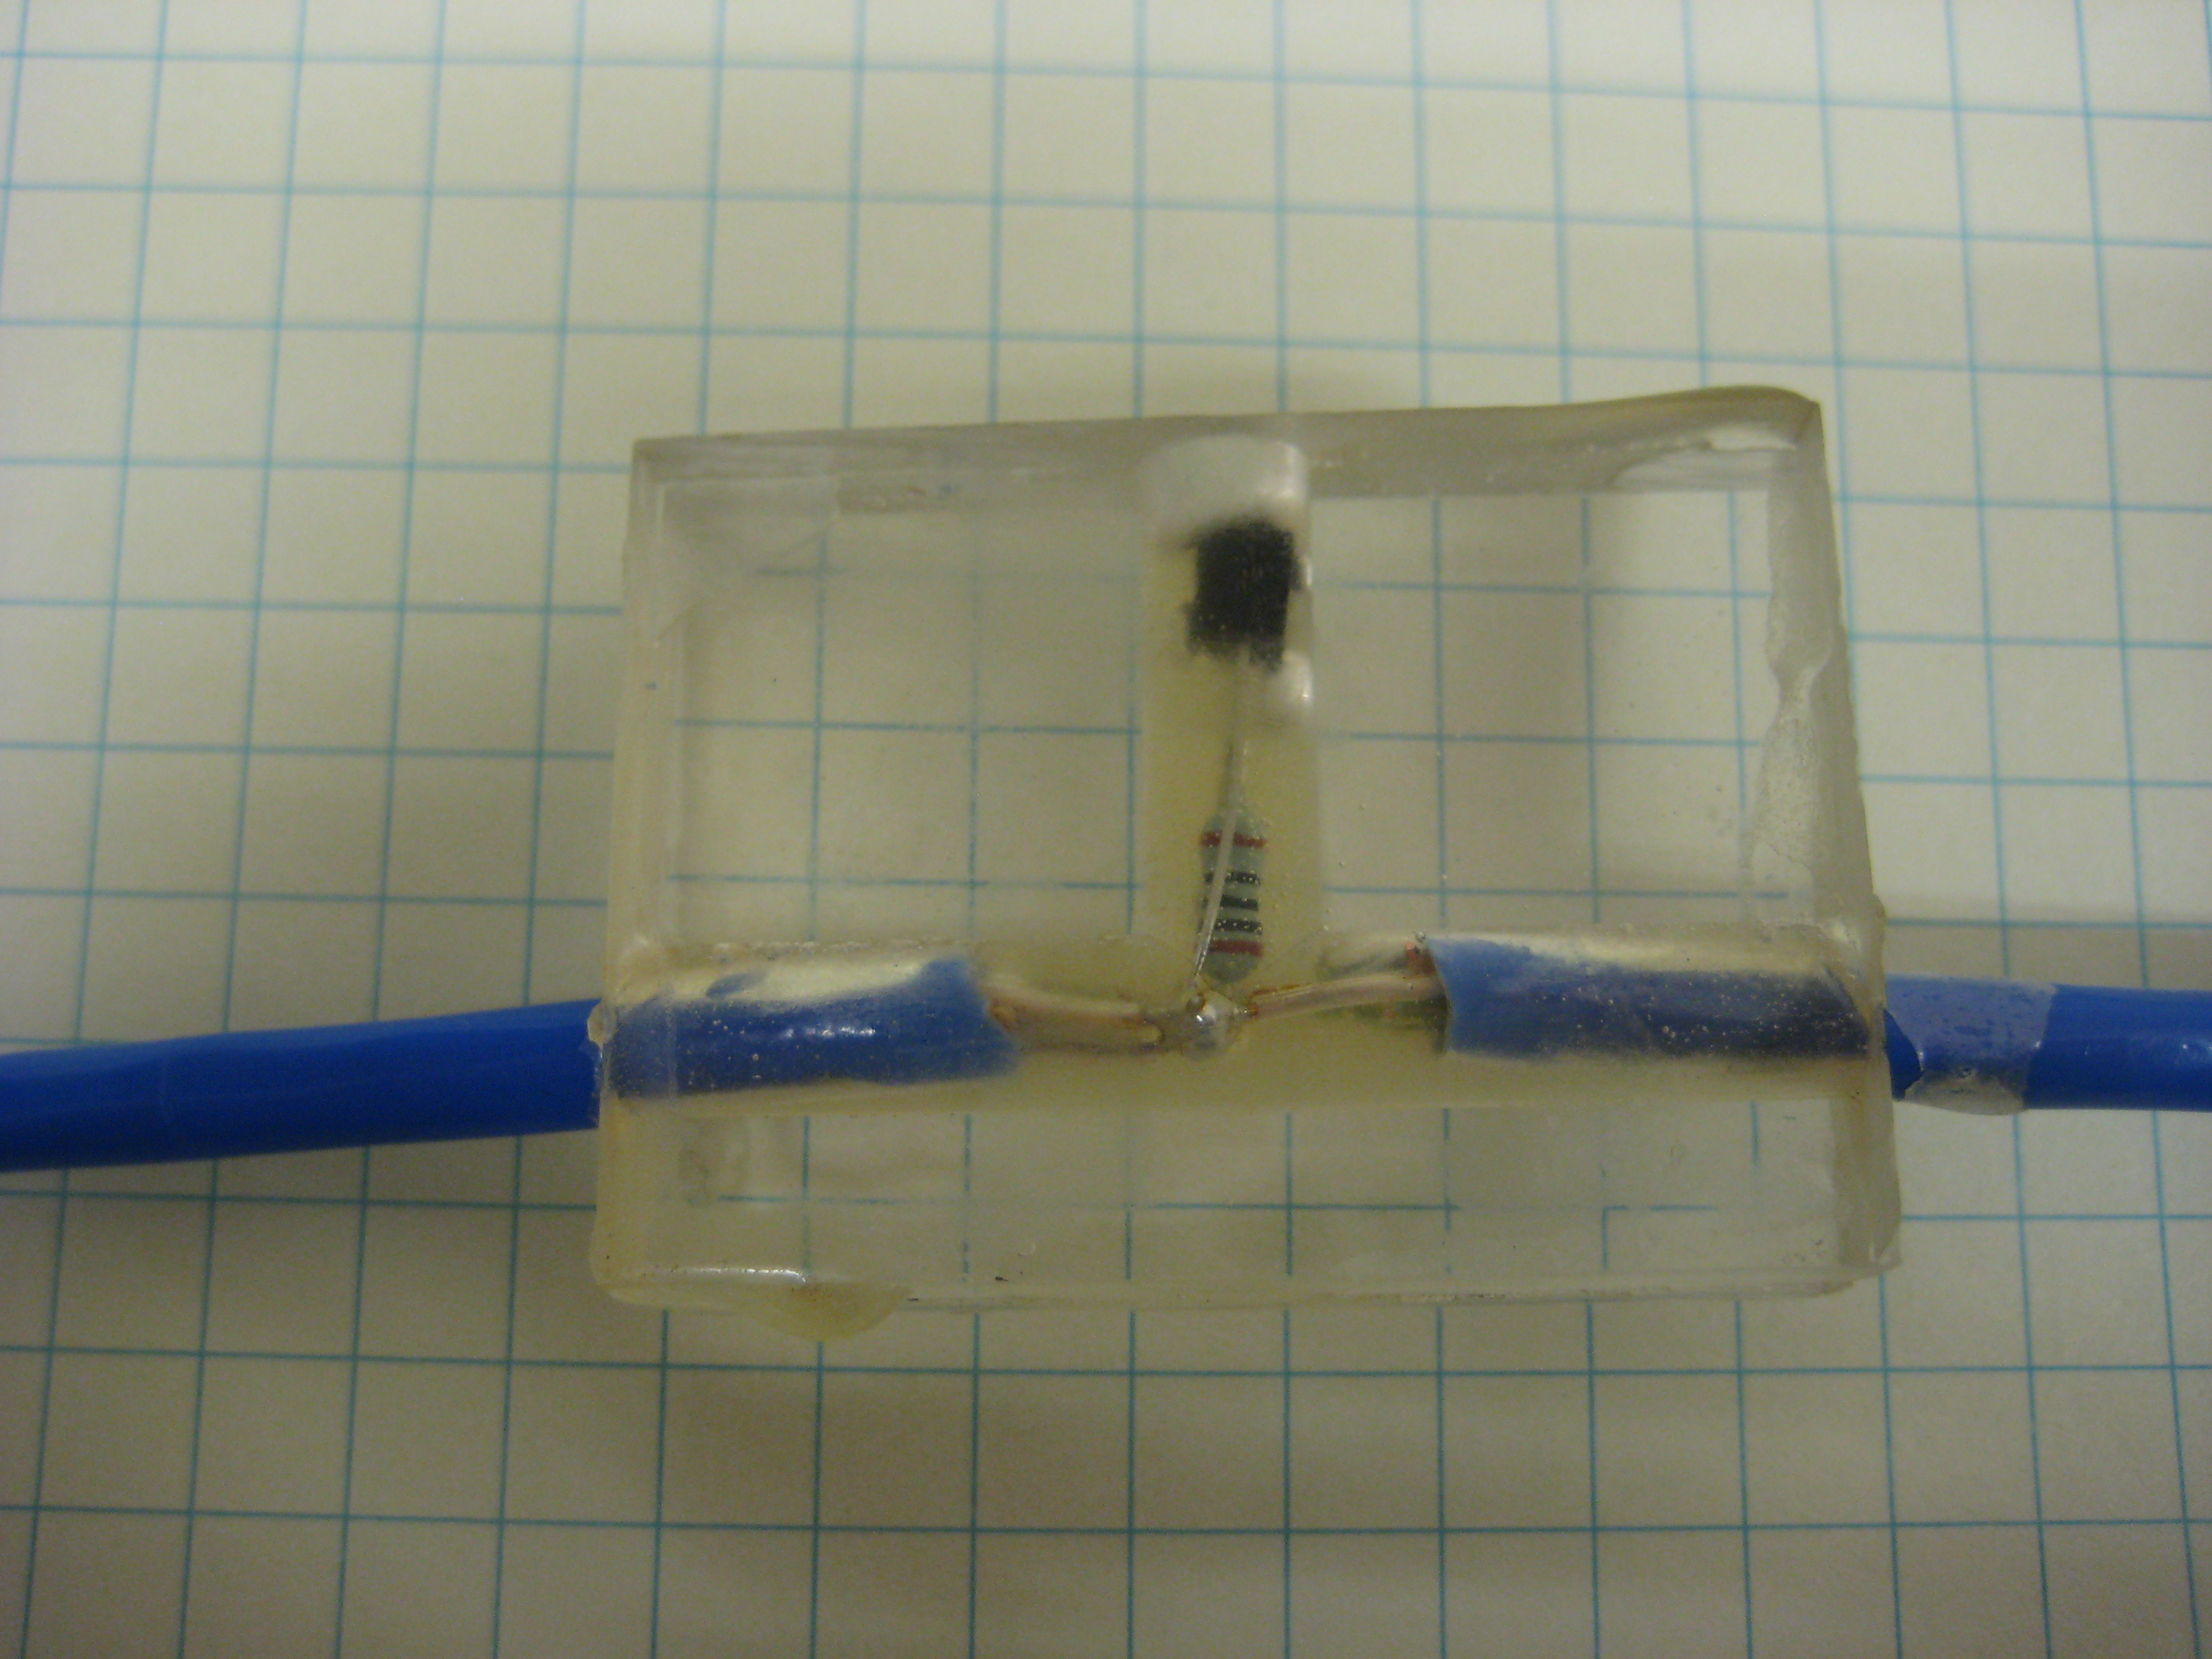
\includegraphics[width=\textwidth]{IMG_2883.JPG}
                \caption{An IVMON prototype.}
                \label{fig4b}
        \end{subfigure}

        \caption{(a) A BMON prototype is sealed in an acrylic box with epoxy. (b) An IVMON prototype is sealed in an acrylic box with epoxy.  }\label{figure4}
\end{figure}

Essentially, the magnetic field in the buffer vessel has maintained a stable status since 2009. However, there were some unusual cases which can observe the magnetic field reduced by a shield design. In 2010, according to an inner veto PMT broken issue, the inner veto lid was opened on April sixth and then closed back on May 21. Figure ~\ref{fig6} shows one example of magnetic field vs. time from BMON no.1 which is mounted on the buffer vessel lid. When the lid was opened, BMON no.1 indicated a obvious change from April to May 2010. After the lid closed, the magnetic field became smaller in two directions. The phenomenon can explain the stainless vessels reduce some certain value of the environmental magnetic field.
\begin{figure}
\centering
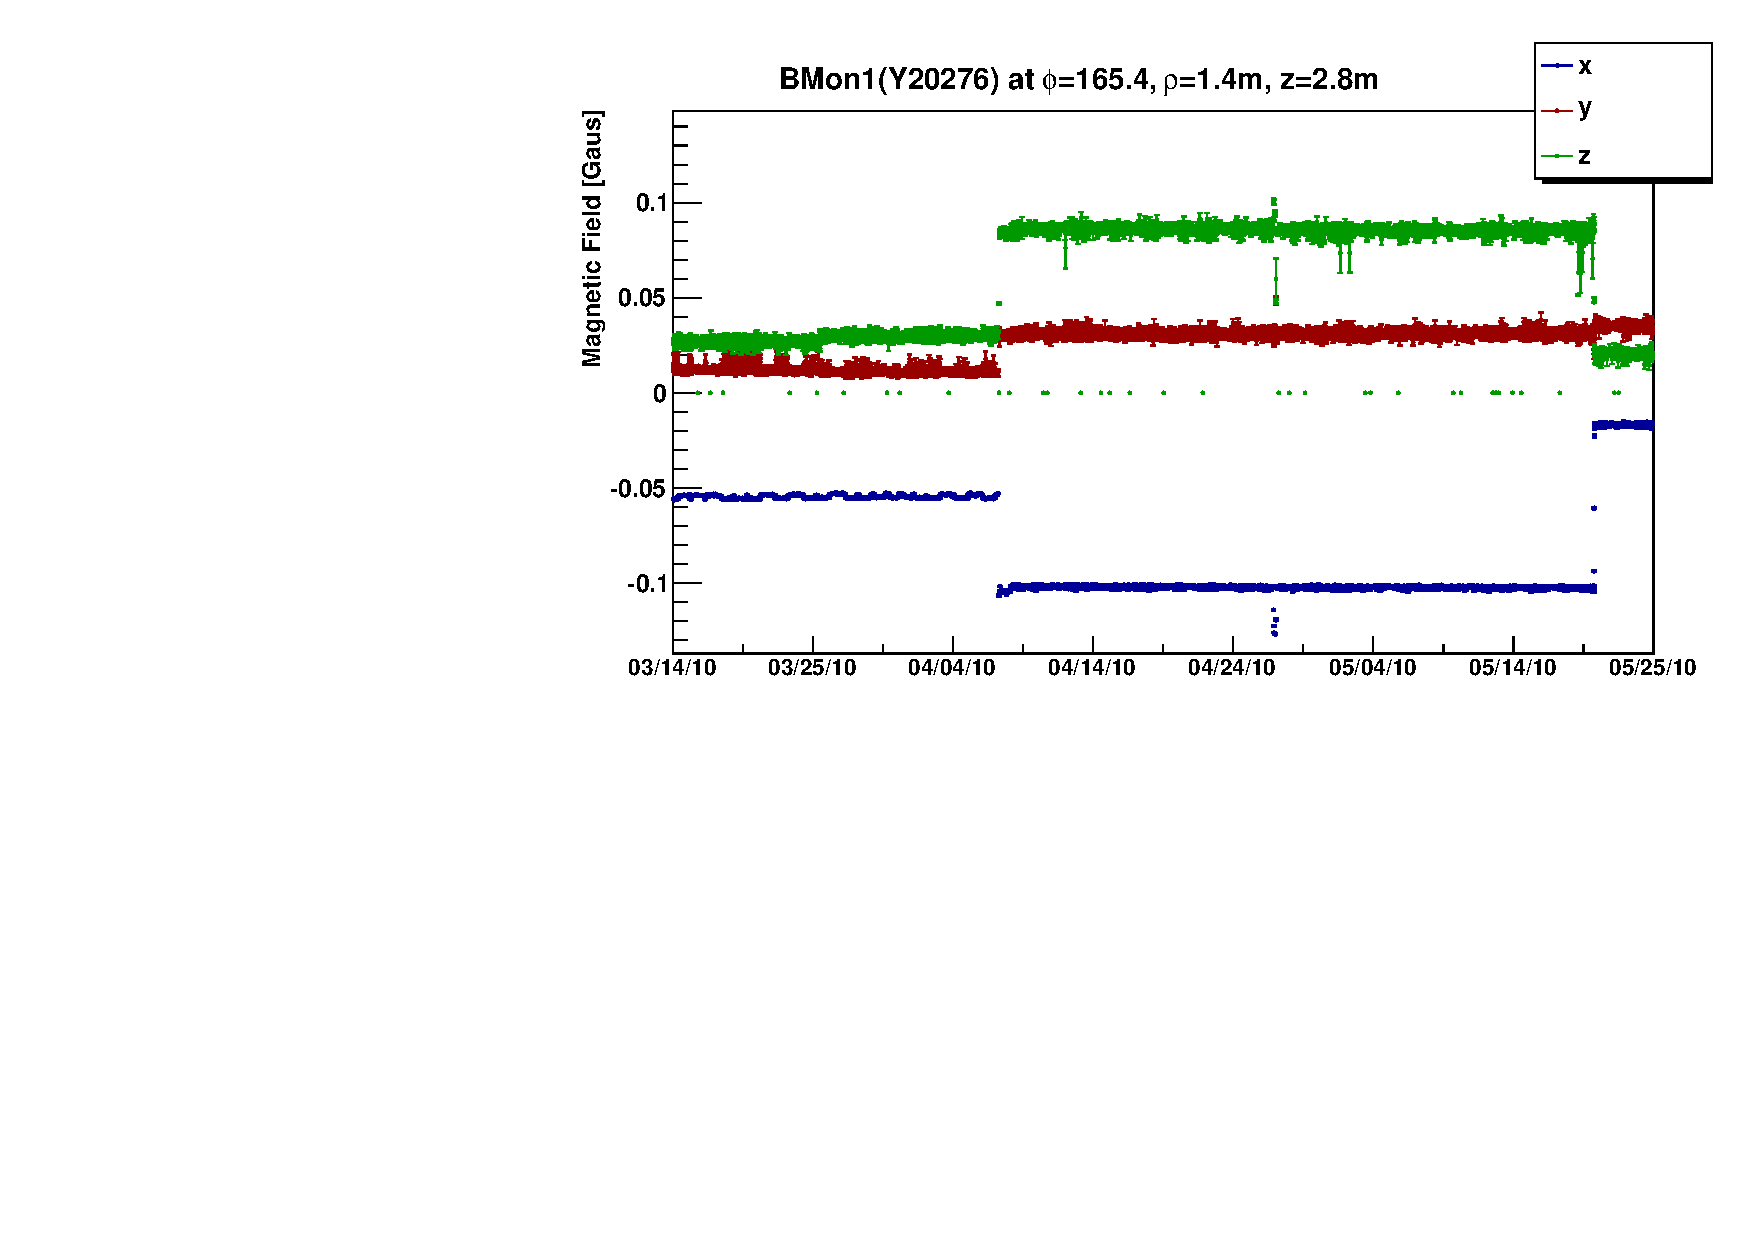
\includegraphics[width=.6\textwidth]{BMon01_MagField_2010-3-15to2010-5-25.pdf}
\caption{BMON no. 1 mounted on the buffer vessel lid is the closest to inner veto vessel lid. Blue dot is X axis, green dot is Y axis and red dot is Z axis. Magnetic fields along X and Y directions can feel strongly change from an obvious stage  when the inner veto vessel lid was opened. However, Z direction didn\textquoteright t return back to the original stable value after the lid was closed.}
\label{fig6}
\end{figure}

The buffer liquid temperature has been waving slightly around 14$\pm$1$^\circ$C with four seasons after finishing the detector installation. According to our experiment, the epoxy thermal mean life time needs 23.81$\pm$0.24 minutes so we collect temperature data from sensors in liquid every ten minutes. The most interesting period was in a filling liquid process which started from October 2010. In the meanwhile, the reading temperature from BMONs suddenly dropped down which presented some stage functions of time in Figure ~\ref{fig7} because sensors have touched the liquid. Some interruptions which caused a liquid thermalization can be easily indicated by an exponential function of time in figure 8. One can easy to get a thermal mean lifetime by fitting an exponential function. For instance, the mean lifetime at the bottom of the buffer vessel is around 8 days in Figure ~\ref{fig8}.
\begin{figure}
\centering
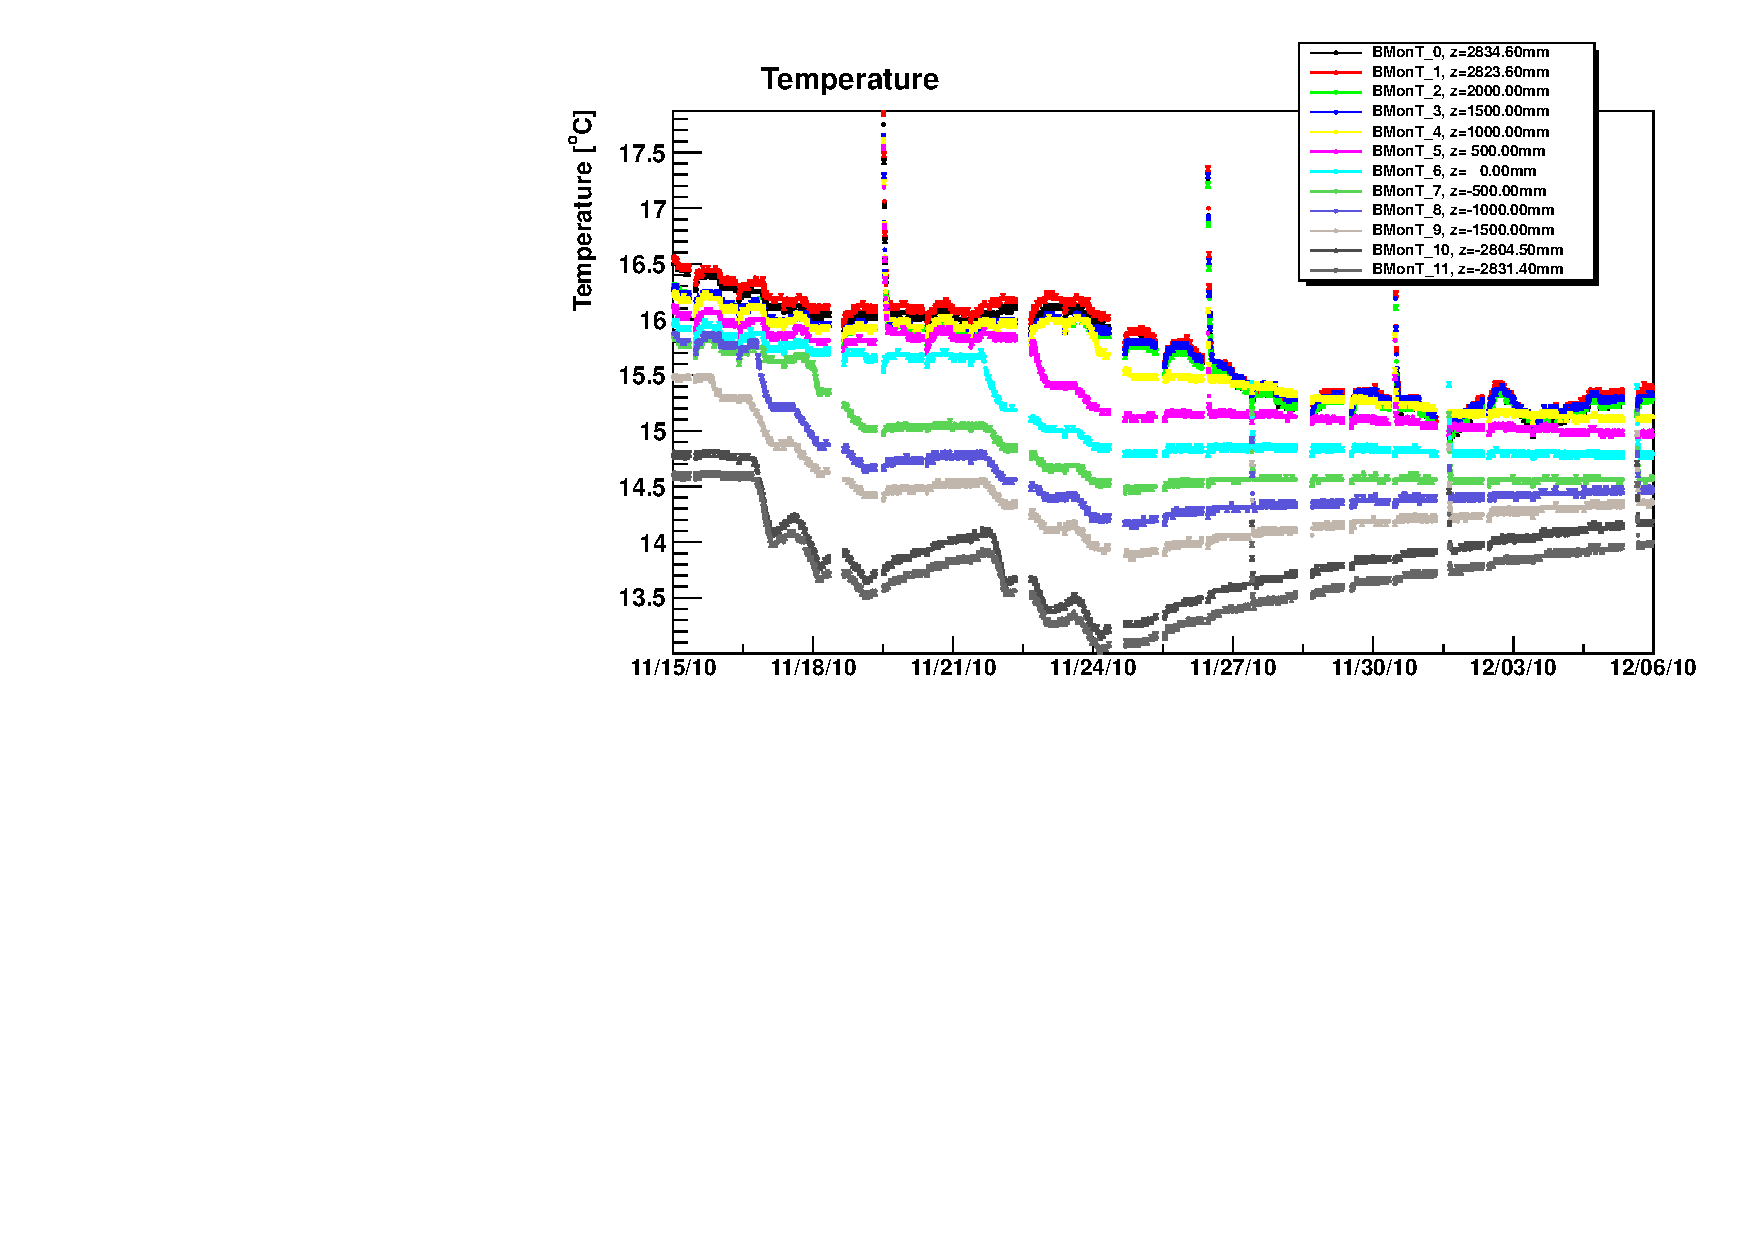
\includegraphics[width=.6\textwidth]{BMonall_Temperature2010-11-15to2010-12-6.pdf}
\caption{This plot is an epitome of the filling process of the Double Chooz far detector. A cooler liquid injected into buffer vessel would cause temperature drop down(stage functions on the figure) BMONs at lower altitude and subsequently interruptions let liquid thermalization(exponential function in figure). After Nov. 24, the liquid in the buffer vessel had been doing thermalization with the latitude and finally the temperature would reach to certain point. There were some BMONs(z>1500mm,z=0 is at the center of detector.) were above the liquid level at that time.}
\label{fig7}
\end{figure}

\begin{figure}
\centering
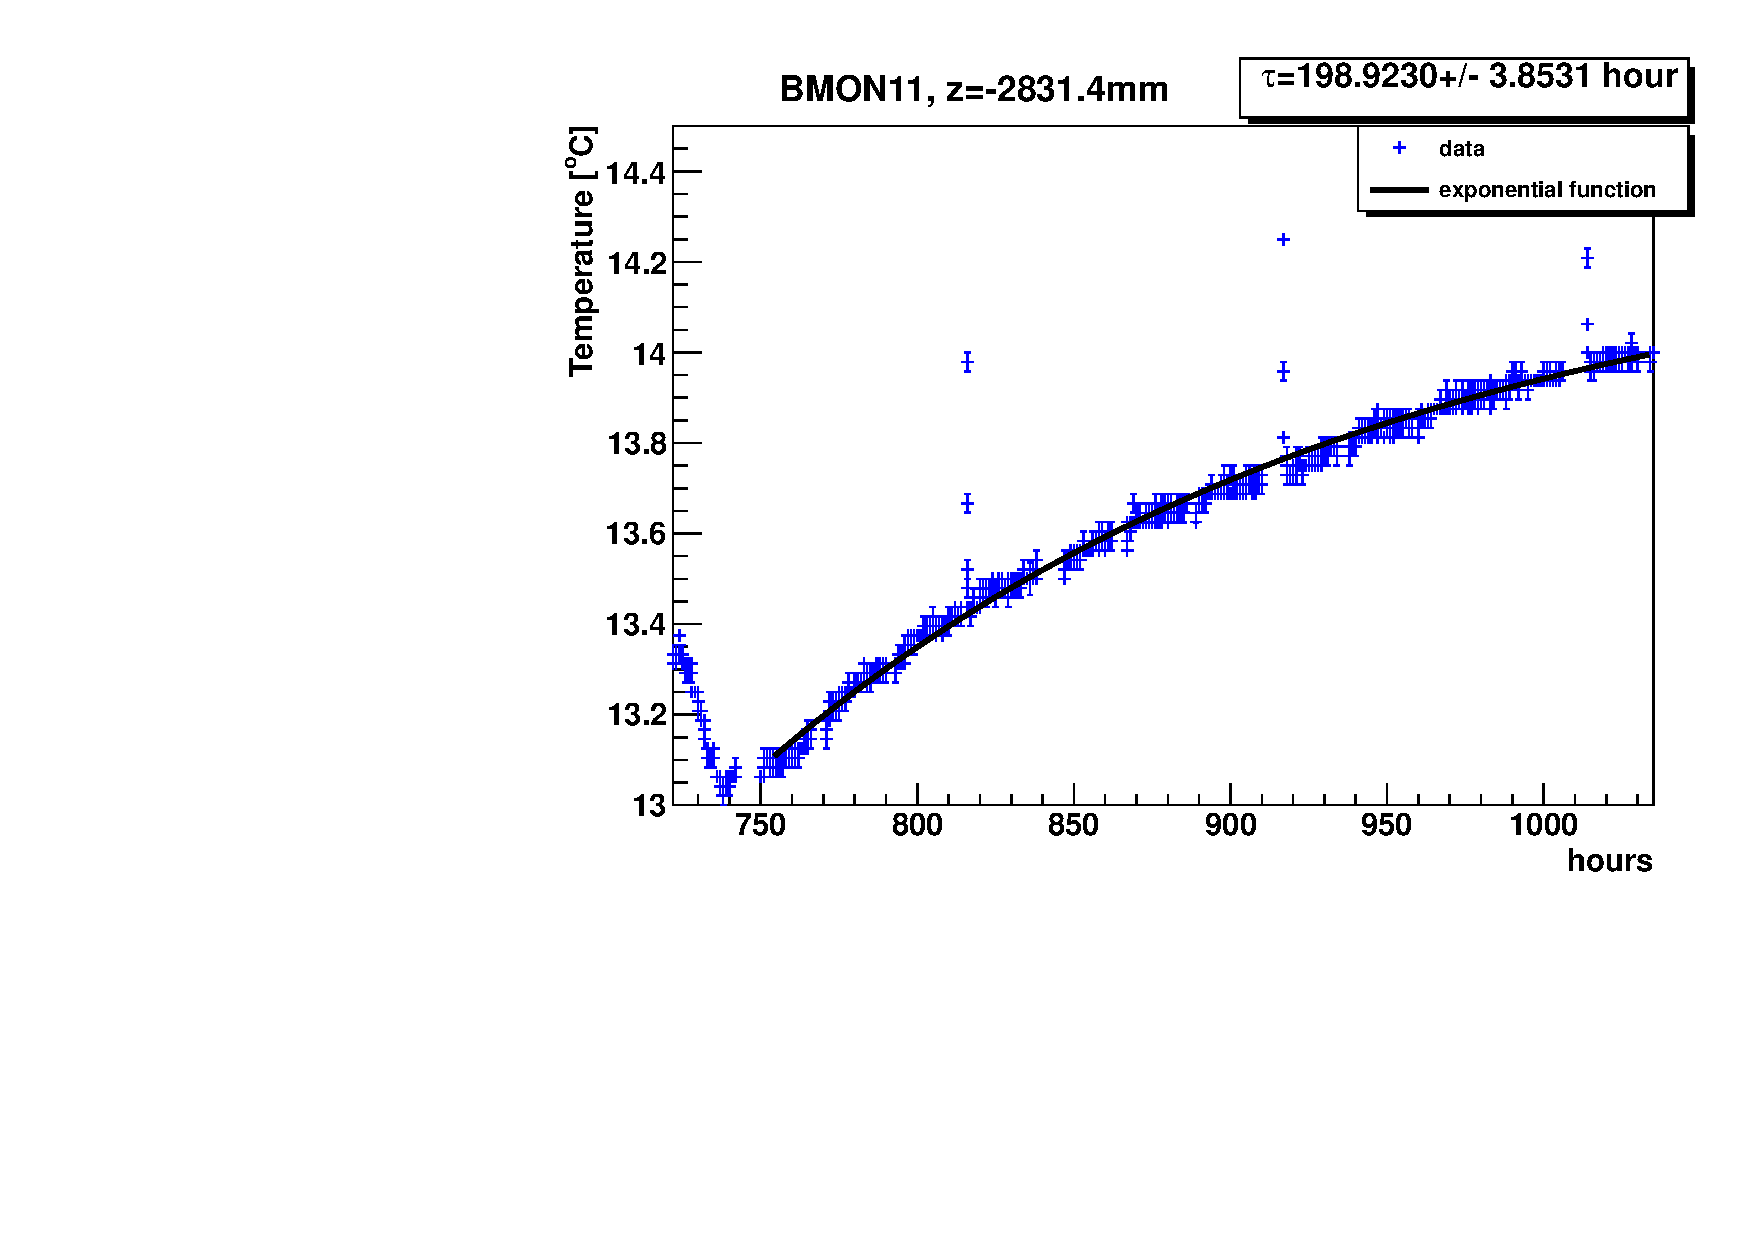
\includegraphics[width=.6\textwidth]{BMONtemp11.pdf}
\caption{This plot is from one of BMONs located at the bottom of the buffer vessel between Nov. 24 and Dec. 7 2010. This period was a very long interruption of the filling process and the buffer vessel was 67\% fill at least. A fill liquid detector could infer a mean life time of $\tau$ 198.92 hours from a fitting of the plot.}
\label{fig8}
\end{figure}

\subsection{Sensors are in air}
The second type sensors are distributed in the laboratory hall to monitor the environmental conditions of the laboratory, a electronics control room and electronics split control boxes and the high voltages of the front-end electronics boards. Main sensors are 82 front-end electronics monitors(FEMON) to watch the high voltages of the front-end electronics(FEE) boards which are located at the electronics control room. Each board has 4 channels, VCC+5, VCC-5, FEE current +6V and FEE current -6V, which are from four non-inverting amplifier circuits.(see Figure ~\ref{fig9}) Additionally, each channel has their own allowable values which can give a feedback when voltages are too high or too low.
 \begin{figure}
\centering
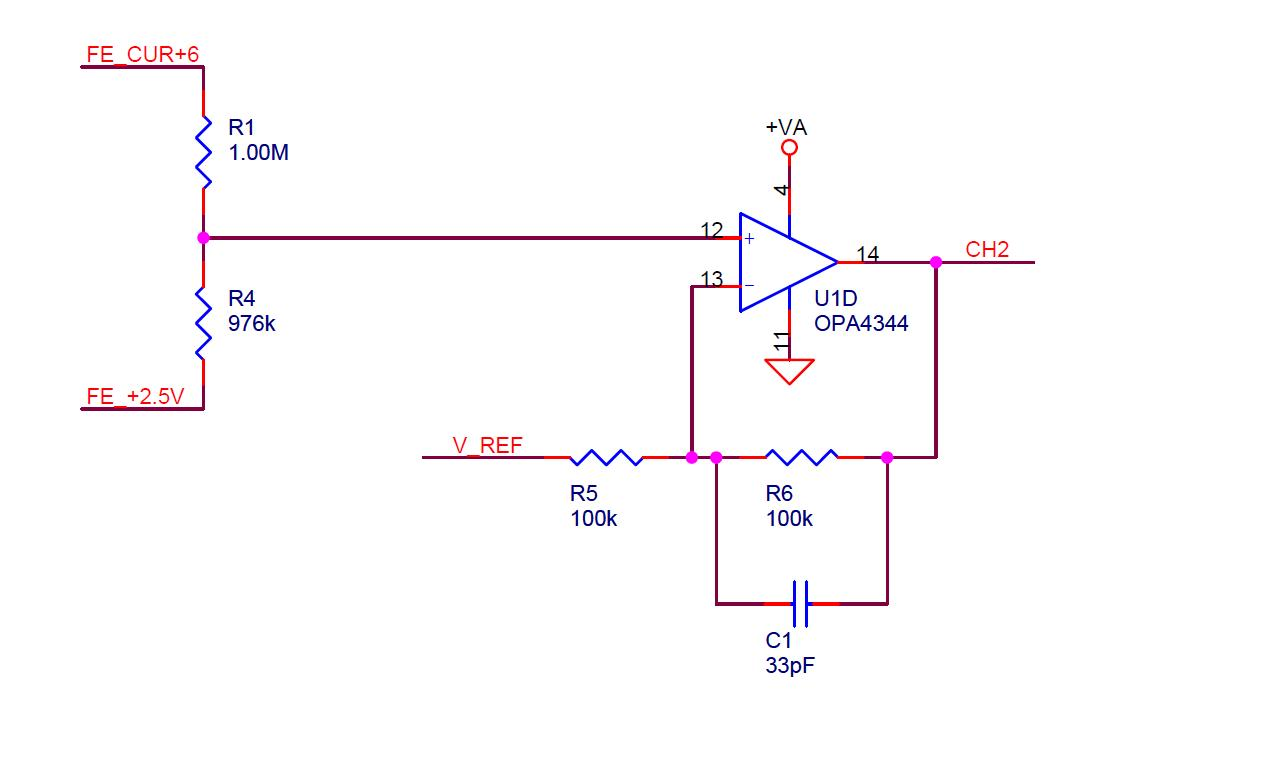
\includegraphics[width=.6\textwidth]{FEMONcir.jpg}
\caption{Schematic layout of partial FEMON.}
\label{fig9}
\end{figure}

Every 7-8 FEMONs are mounted on the same link crate which is monitored by a thermometer. The voltage and temperature values will be update every 10 second. The humidity and temperature are important factors to cause damages on electronics boards so a multi-function sensor, iButton\cite{bib9}, including temperature and humidity is installed in the electronics control room, the laboratory hall and electronics split control boxes. Figure ~\ref{fig10a} and ~\ref{fig10b} are prototypes of FMON and iButton. An online interface panel for shifters is showed in Figure ~\ref{fig12}. Each link crate has a RJ-11 modular phone jack box mounted a thermometer to converge 1-wire devices data and ground wires (see Figure ~\ref{fig13}) back to an USB interface.


\begin{figure}
        \centering
        \begin{subfigure}[b]{0.5\textwidth}
                \centering
                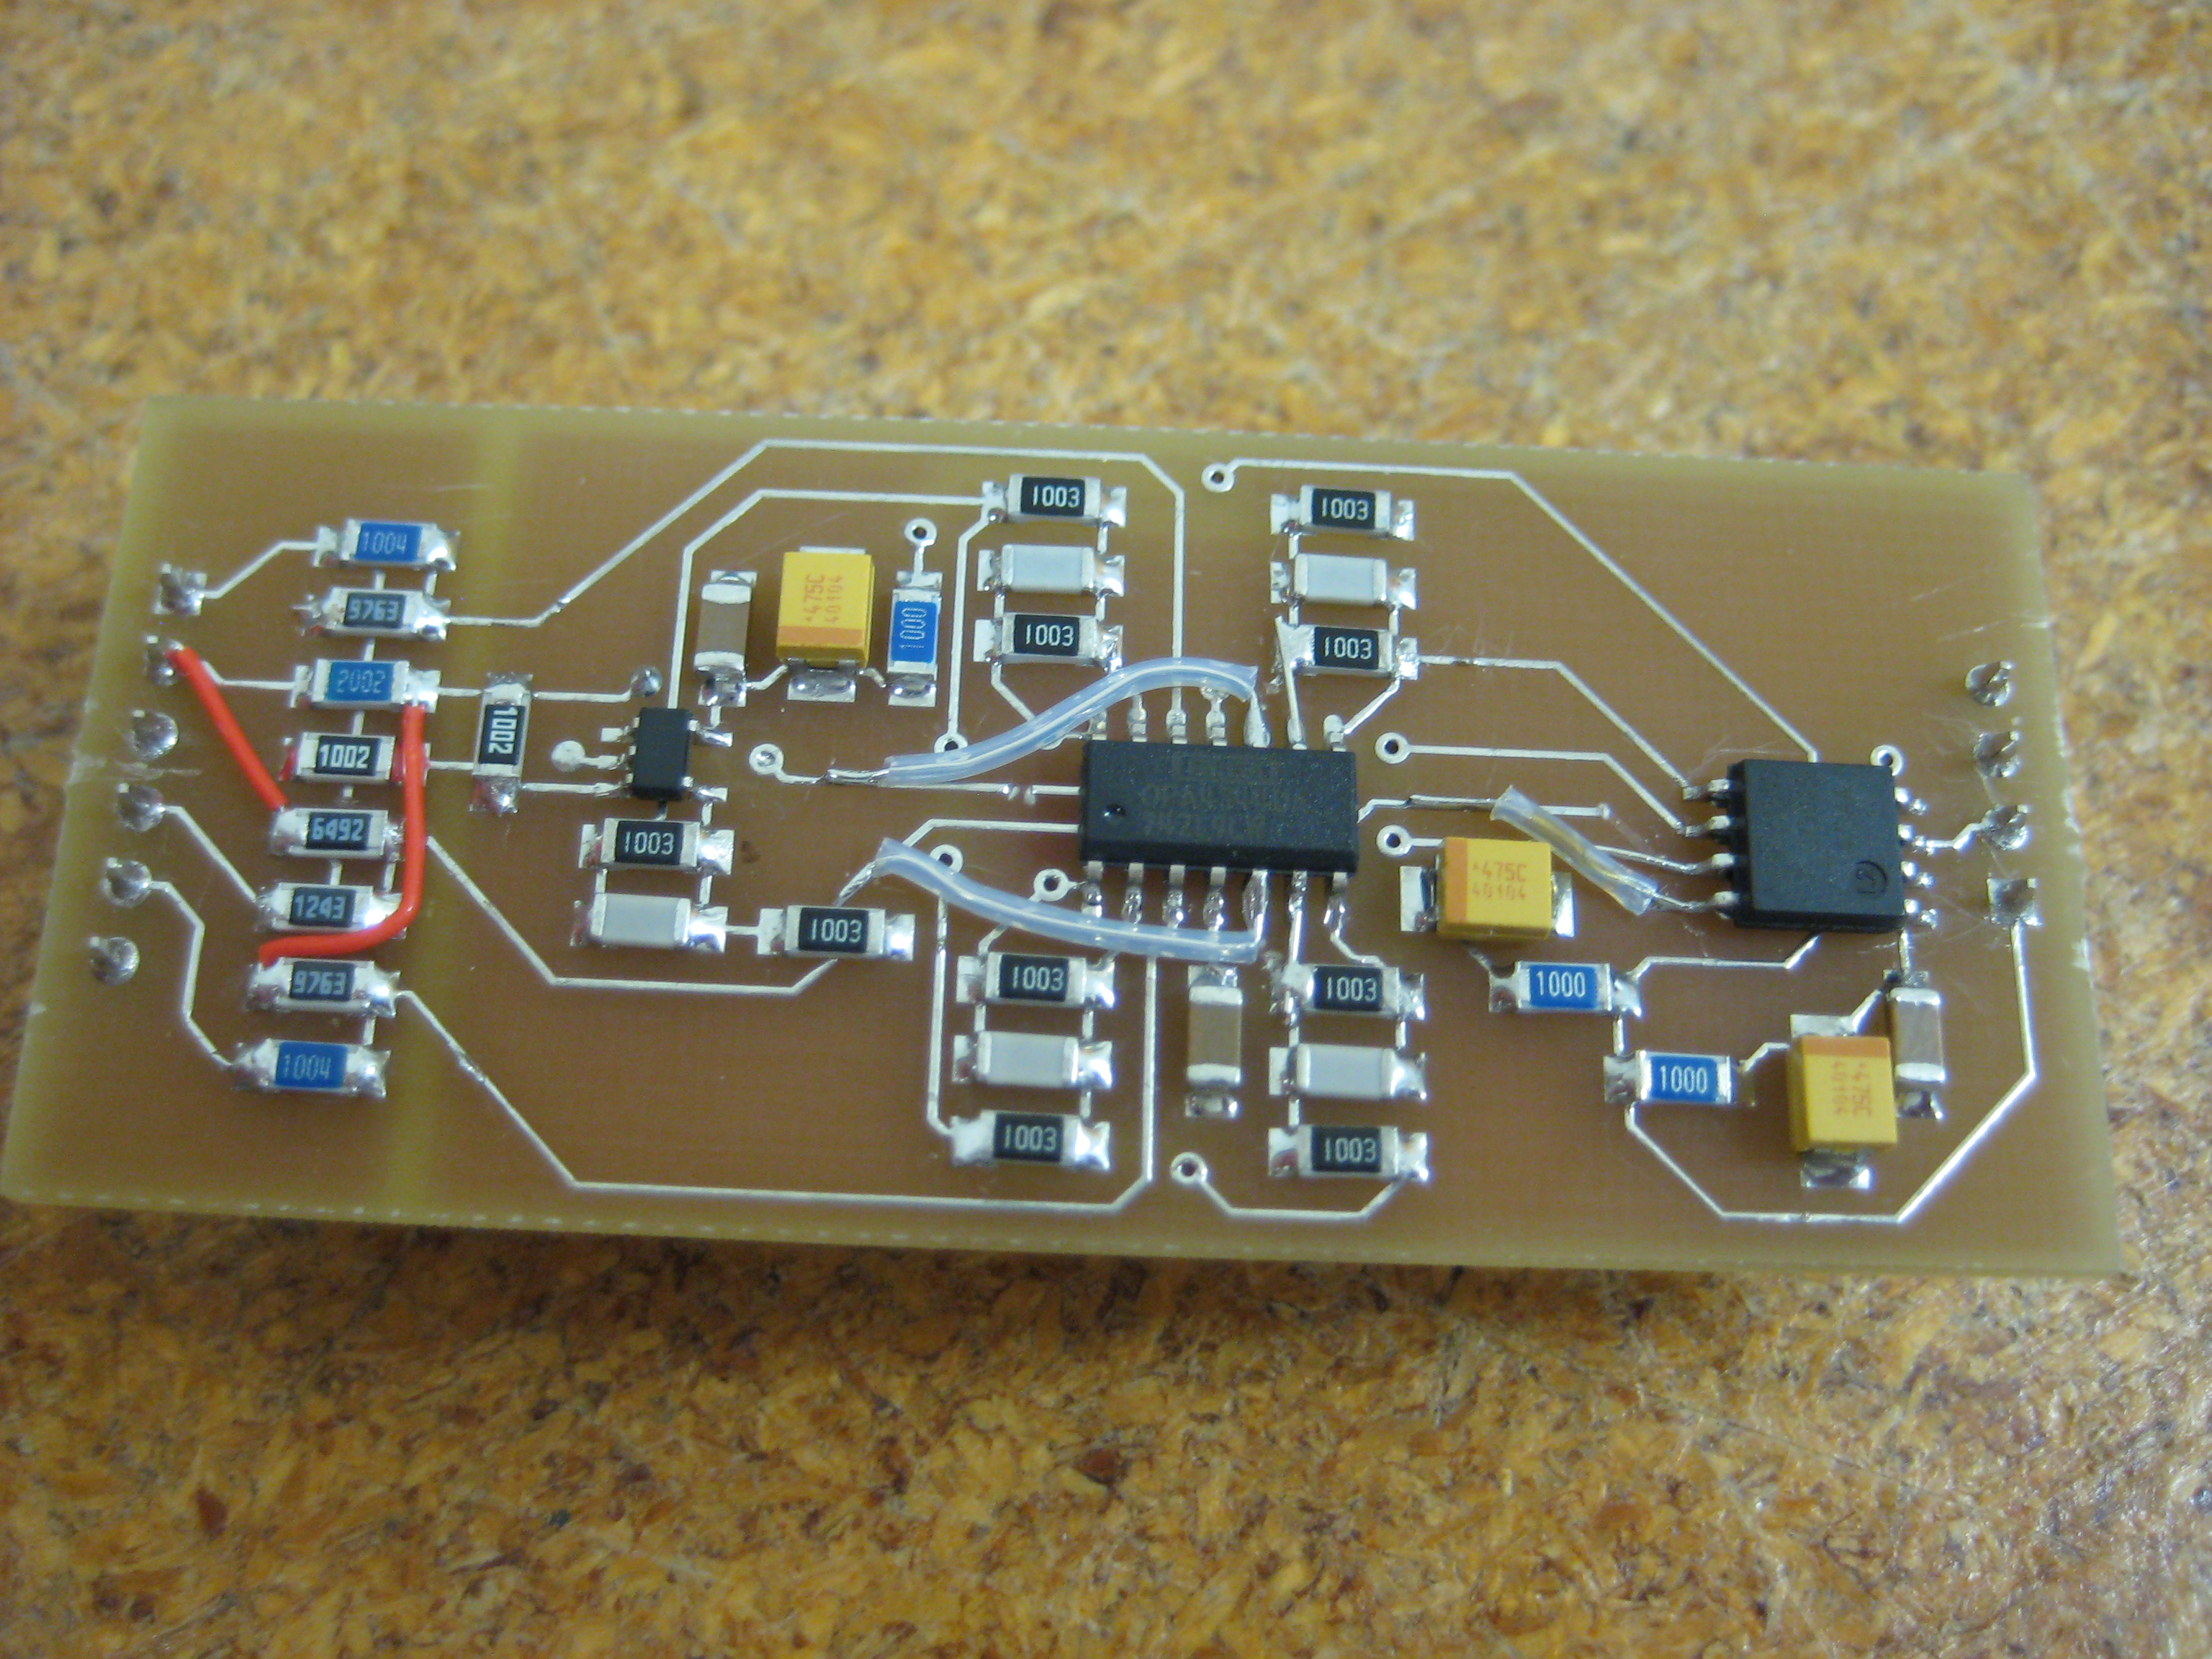
\includegraphics[width=\textwidth]{IMG_3544.JPG}
                \caption{FEMON prototype.}
                \label{fig10a}
        \end{subfigure}%
        ~ %add desired spacing between images, e. g. ~, \quad, \qquad etc.
          %(or a blank line to force the subfigure onto a new line)
        \begin{subfigure}[b]{0.5\textwidth}
                \centering
                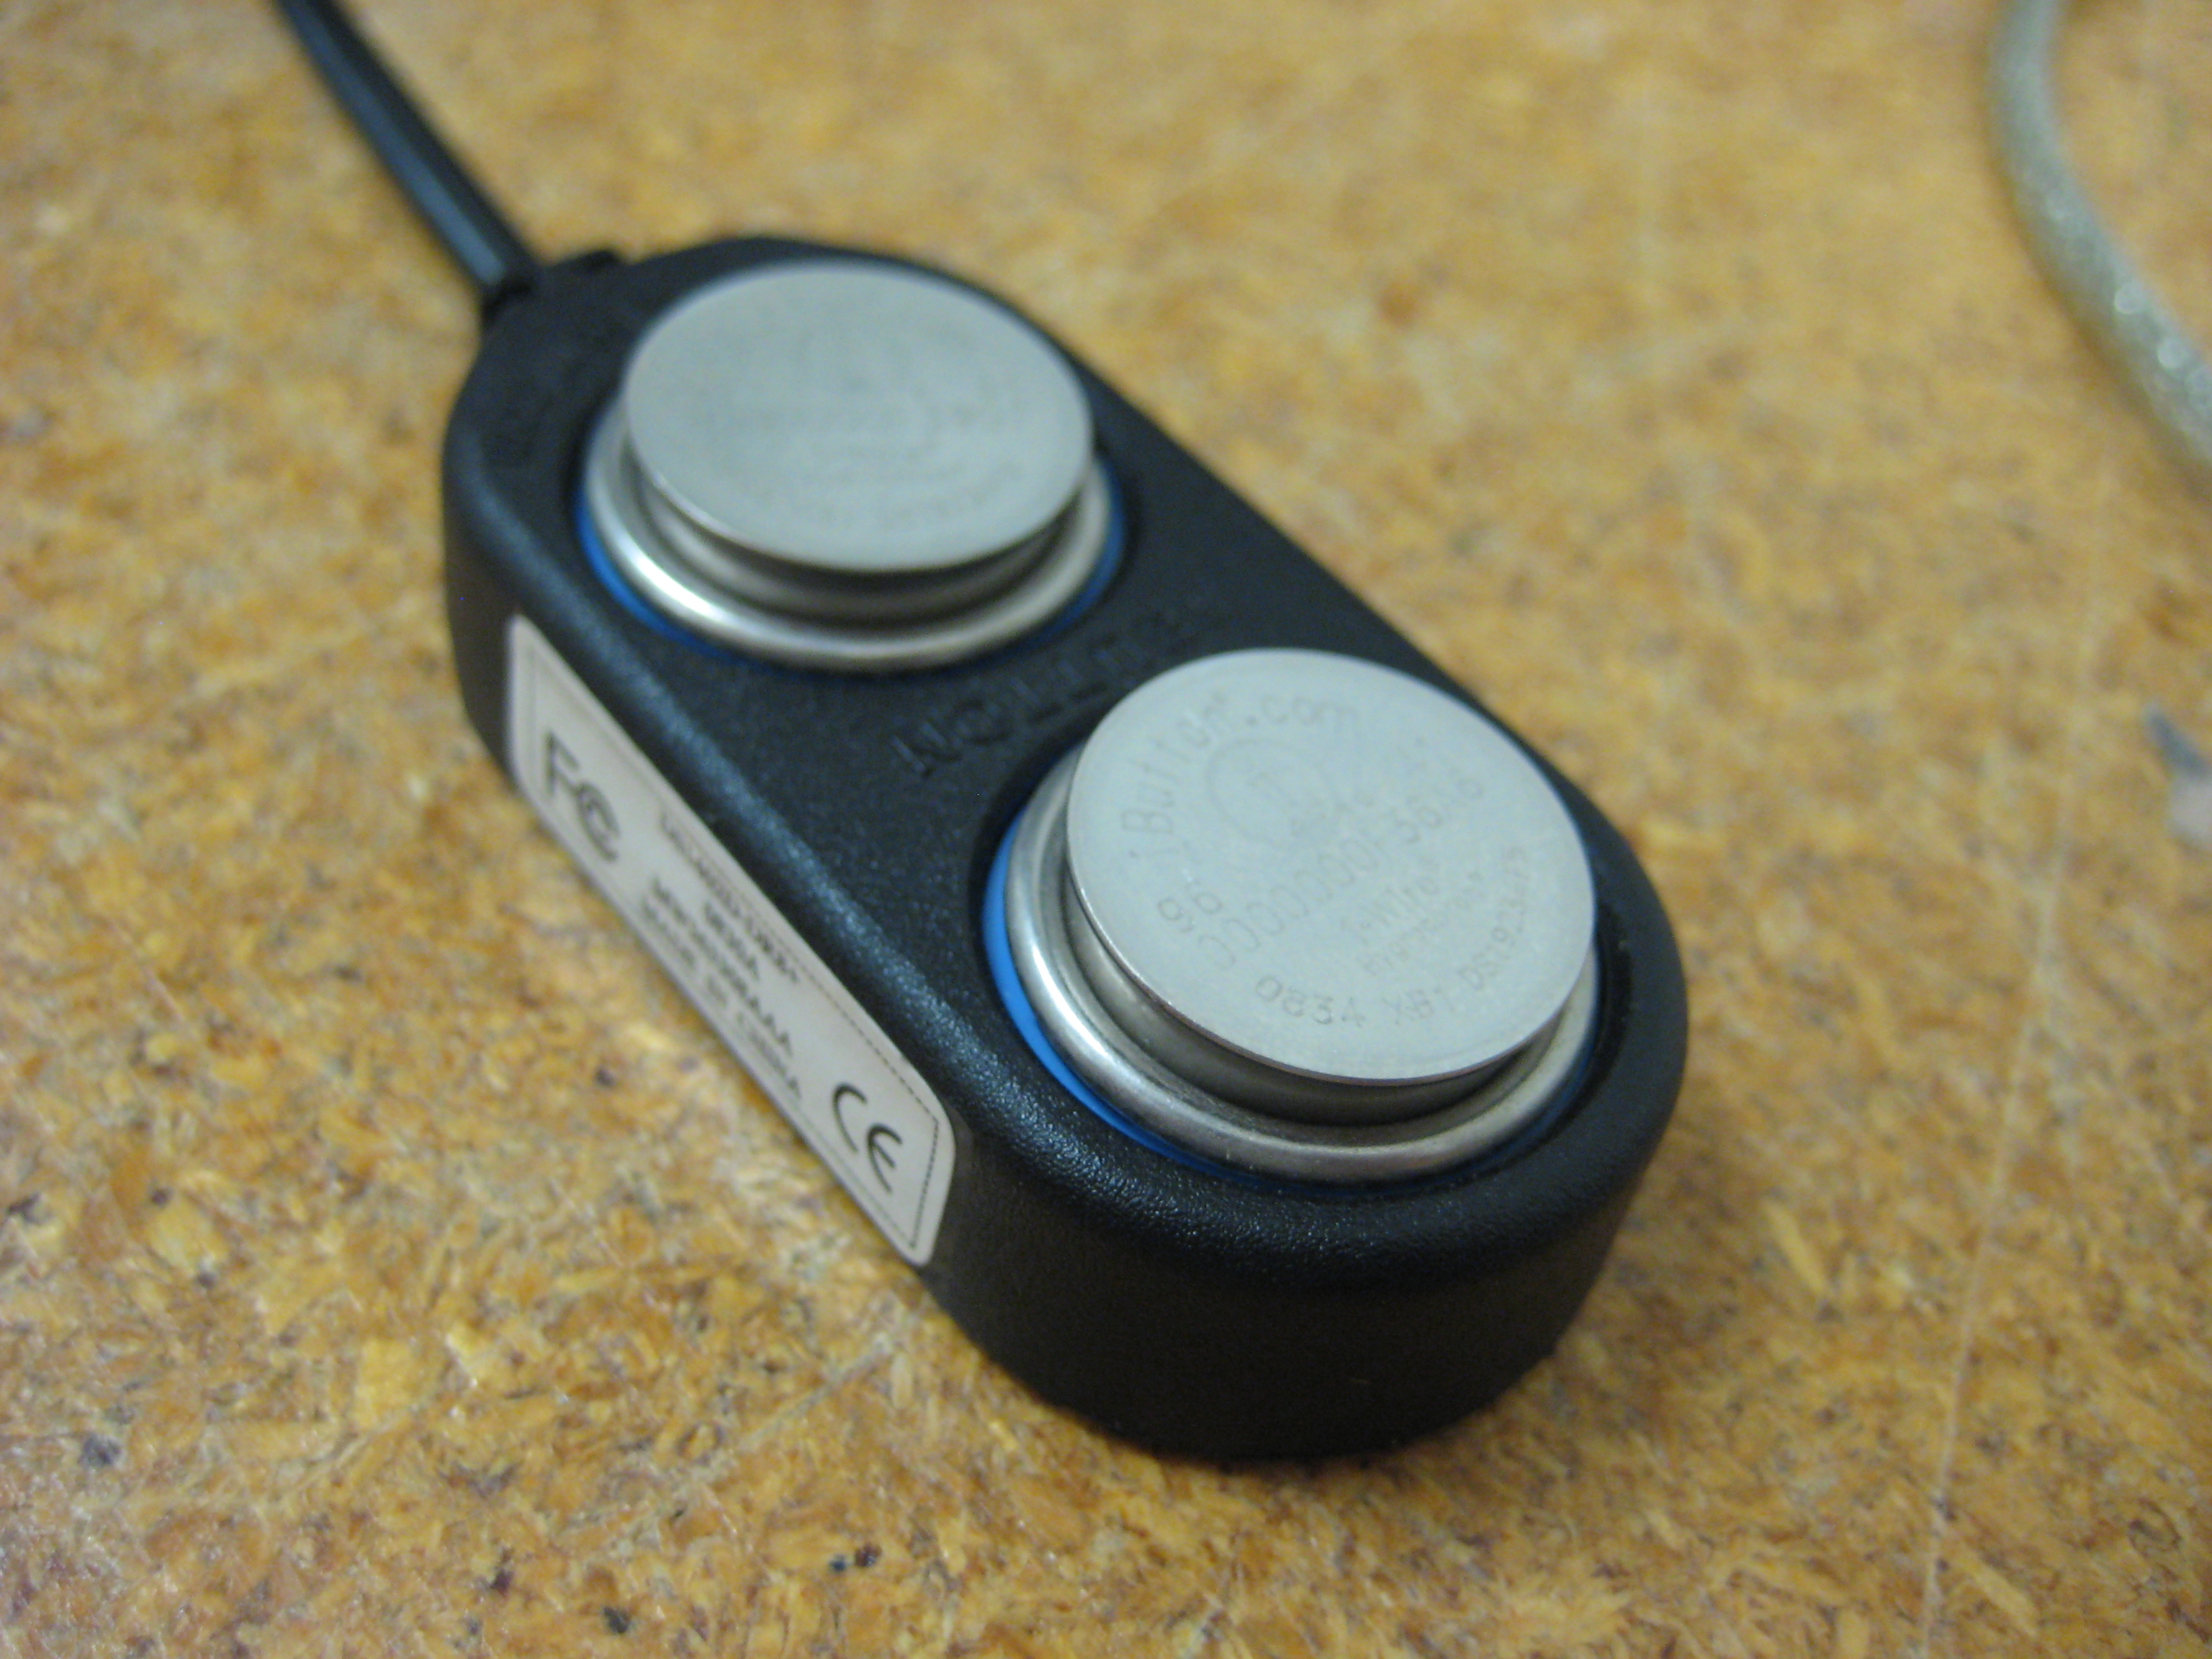
\includegraphics[width=\textwidth]{IMG_3542.JPG}
                \caption{iButton sensors.}
                \label{fig10b}
        \end{subfigure}

        \caption{(a) One of the FEMON prototypes. (b) Two of the iButton sensors.  }\label{figure10}
\end{figure}
\begin{figure}
\centering
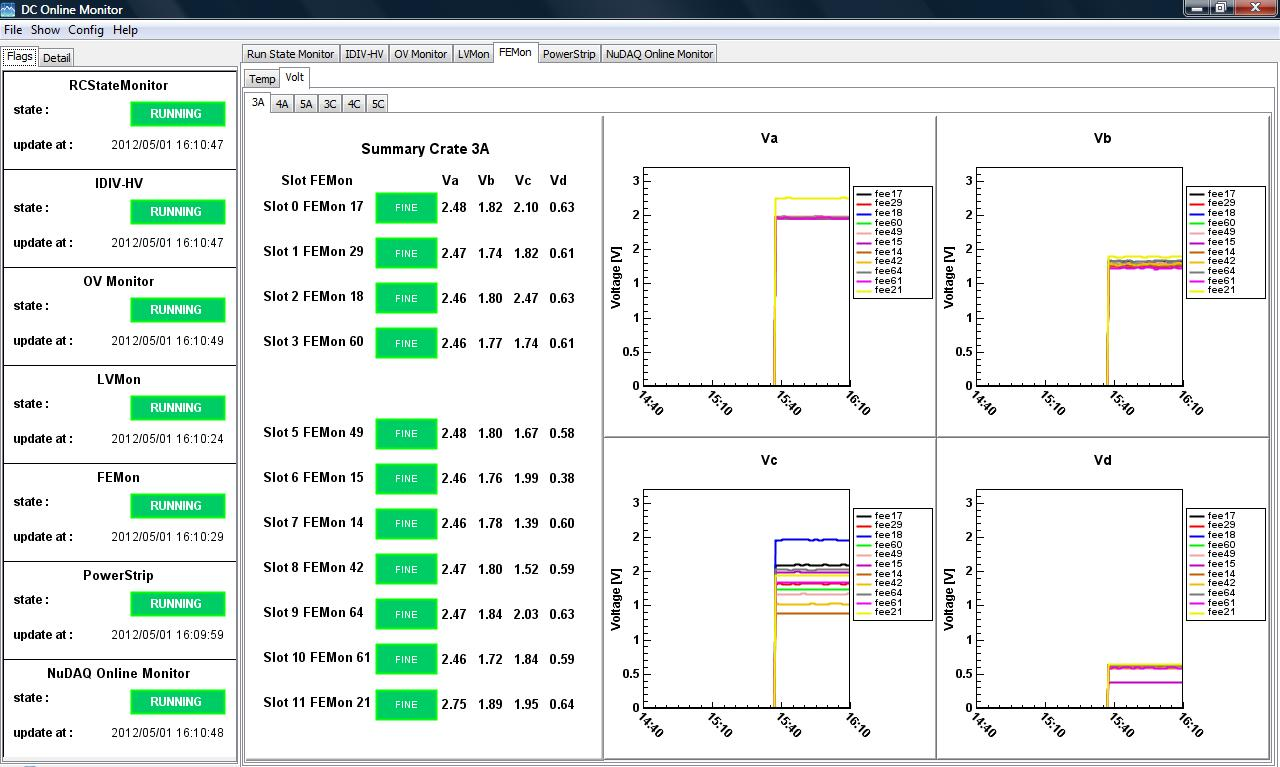
\includegraphics[width=.6\textwidth]{DC.jpg}
\caption{This is a control panel of the data acquisition and control system. This page shows FEMON voltage plots and a shifter could notice positions of problem FEMONs once green boxes become red.}
\label{fig12}
\end{figure}
\begin{figure}
\centering
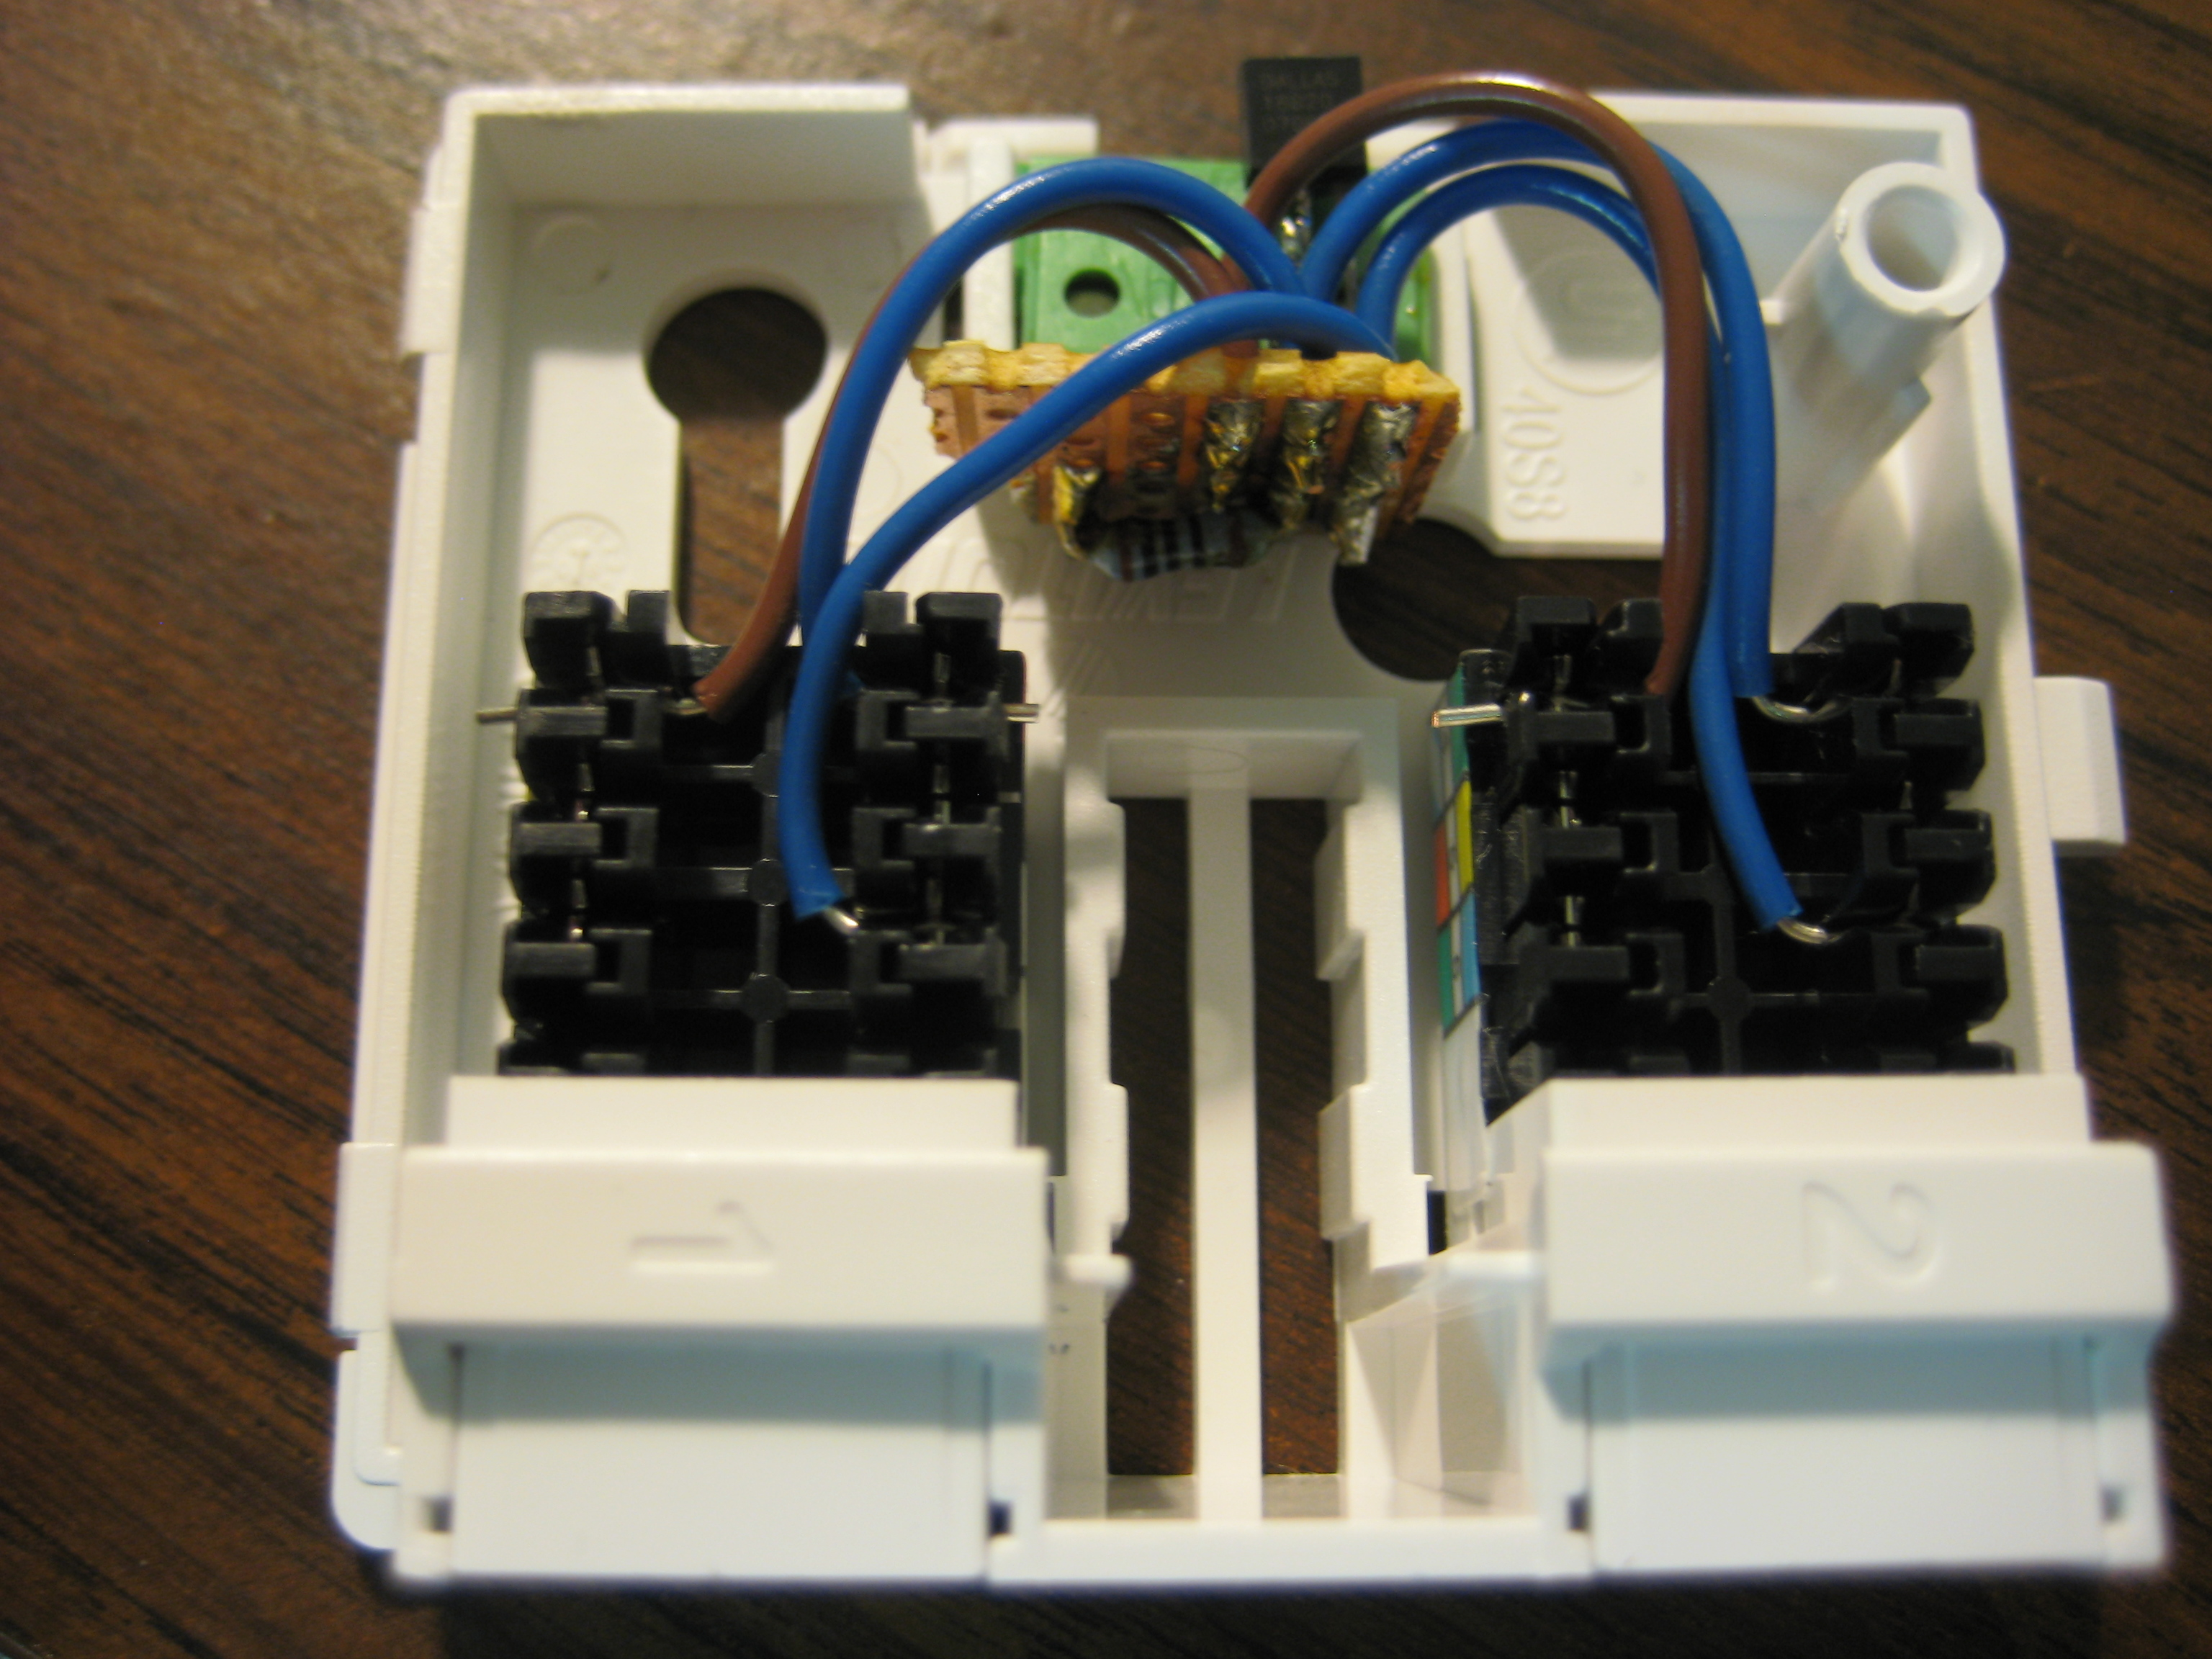
\includegraphics[width=.4\textwidth]{IMG_3649.JPG}
\caption{This is a RJ-11 modular phone jack box. It could converge all FEMON 1-Wire data and ground lines back to a USB port and is also a thermometer to monitor the link crate temperature.}
\label{fig13}
\end{figure}
\section{Radioactivity}
To ensure that the ambitious sensitivity goal of the Double Chooz experiments is attained, great care must be taken to keep the background trigger rate below a few Hz. This requires that a great care is taken in material selection. The background problem of environment monitoring system is from isotopes radioactivity in all sensor assemblies and cables sunk in the liquid. The amount of isotopes are listed in Table ~\ref{tab1} which is from LBNL Berkeley Low Background Facility (Nathaniel Bowden and Allan R. Smith).

\begin{table}
\caption{Isotope amount in a BMON and cables} % title of Table
\centering  % used for centering table
\begin{tabular}{c c c } % centered columns (4 columns)
\hline\hline                        %inserts double horizontal lines
isotope& ppm(sensors)&ppm(cables)\\ [0.5ex] % inserts table
%heading
\hline                  % inserts single horizontal line
$^{238}U$ & 0.085(6)& <0.007   \\ % inserting body of the table
$^{232}Th$  & 0.40(2)  & <0.015 \\
$^{40}K$  & <20 & 27(3) \\ [1ex]      % [1ex] adds vertical space
\hline %inserts single line
\end{tabular}
\label{tab1} % is used to refer this table in the text
\end{table}

The trigger rate from isotopes can be simulated by Monte Carlo (MC) based on Geant4 to reconstruct a detector model. The orientation of BMONs is simulated with two different ways. One is that the sensors forward to the buffer vessel wall(see Figure ~\ref{fig14a} and ~\ref{fig14b}) and the other one is at opposite direction.

%\begin{figure}
%\centering
%\begin{minipage}{16pc}
%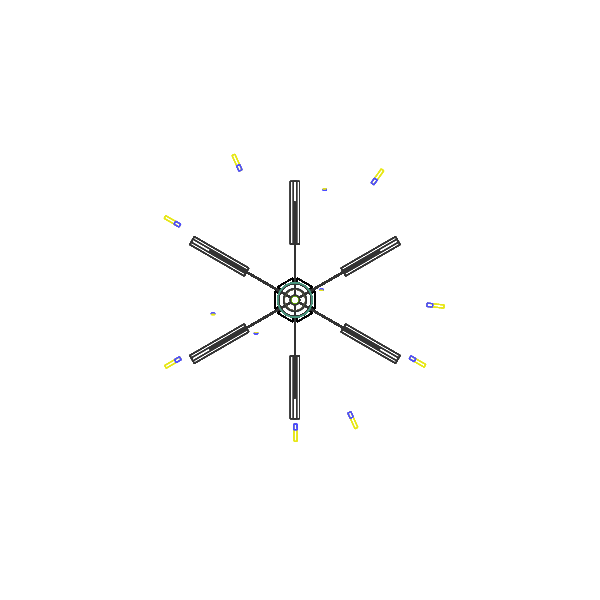
\includegraphics[width=16pc]{bmon_positions_XY_in.png}
%\caption{The distribution of BMONs at X-Y intersection of detector. Blue square is sensor and yellow is acrylic base plates.}
%\label{fig14}
%\end{minipage}\hspace{2pc}%
%\begin{minipage}{16pc}
%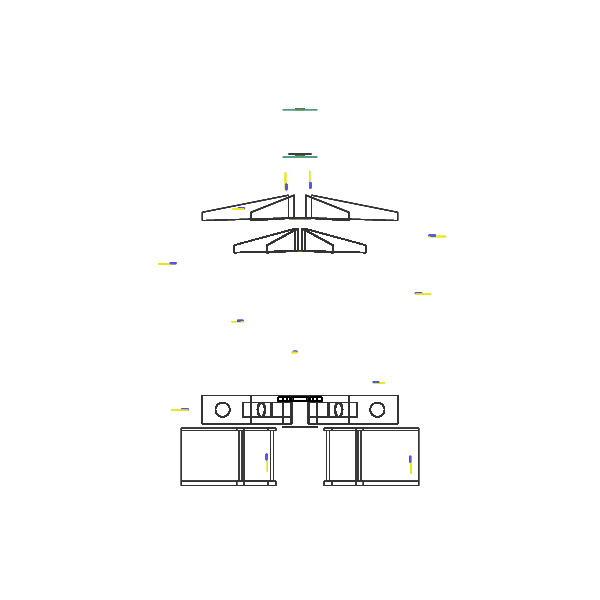
\includegraphics[width=16pc]{bmon_positions_YZ_in.png}
%\caption{The distribution of BMONs at Z intersection of detector. Blue square is sensor and yellow is acrylic base plates.}
%\label{fig15}
%\end{minipage}
%\end{figure}


\begin{figure}
        \centering
        \begin{subfigure}[b]{0.5\textwidth}
                \centering
                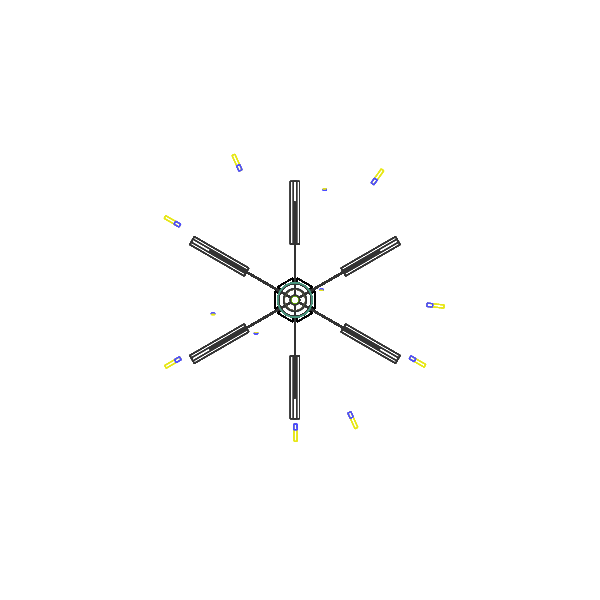
\includegraphics[width=\textwidth]{bmon_positions_XY_in.png}
                \caption{ The distribution of BMONs at X-Y intersection.}
                \label{fig14a}
        \end{subfigure}%
        ~ %add desired spacing between images, e. g. ~, \quad, \qquad etc.
          %(or a blank line to force the subfigure onto a new line)
        \begin{subfigure}[b]{0.5\textwidth}
                \centering
                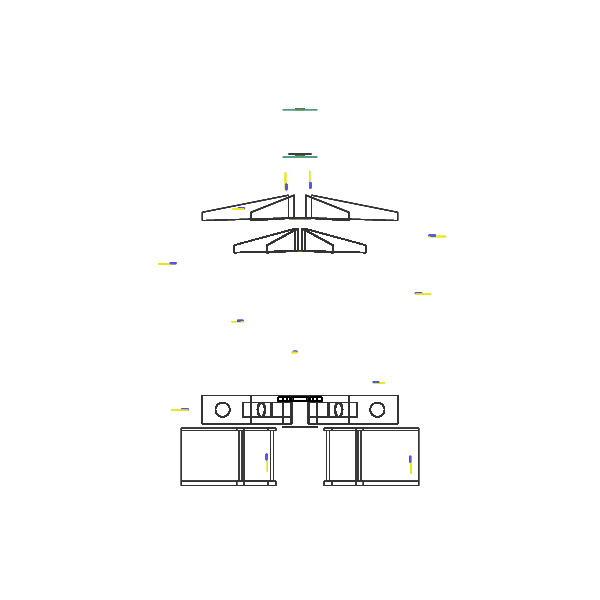
\includegraphics[width=\textwidth]{bmon_positions_YZ_in.png}
                \caption{The distribution of BMONs at Z intersection.}
                \label{fig14b}
        \end{subfigure}

        \caption{(a) The distribution of BMONs at X-Y intersection of detector. (b) The distribution of BMONs at Z intersection of detector. Blue square is sensor and yellow is acrylic base plates.  }\label{figure14}
\end{figure}

The orientation of the sensors pointing away from the wall got smaller trigger rates from the simulation and the result is shown at Table~\ref{tab2}. Assuming all cables are distributed uniformly in the detector and we can propose a 0.5 mm thick painting model to simulate the trigger rates from isotopes with MC. The painting model result is shown in Table~\ref{tab3}. According to the simulation results ,the total accidental trigger rate is small than 0.1 Hz from sensors in the liquid. Comparing to nature background from muon and PMT isotopes, physical environmental system radioactivity is not a main issue.
\begin{table}
\caption{The simulation of trigger rates from BMONs.} % title of Table
\centering  % used for centering table
\begin{tabular}{c c c c} % centered columns (4 columns)
\hline\hline                        %inserts double horizontal lines
isotope& E>0.5MeV(Hz)&E>0.7MeV(Hz)&E>0.9MeV(Hz)\\ [0.5ex] % inserts table
%heading
\hline                  % inserts single horizontal line
$^{238}U$ & 0.031&0.028&0.0168    \\ % inserting body of the table
$^{232}Th$  &0.0655   &0.0492 &0.0372 \\
$^{40}K$  & 0.00384 &0.003 & 0.00216\\ [1ex]      % [1ex] adds vertical space
\hline %inserts single line
\end{tabular}
\label{tab2} % is used to refer this table in the text
\end{table}
\begin{table}
\caption{The simulation of trigger rates from cables.} % title of Table
\centering  % used for centering table
\begin{tabular}{c c c c} % centered columns (4 columns)
\hline\hline                        %inserts double horizontal lines
isotope& E>0.5MeV(Hz)&E>0.7MeV(Hz)&E>0.9MeV(Hz)\\ [0.5ex] % inserts table
%heading
\hline                  % inserts single horizontal line
$^{238}U$ & 0.00018&0.000132&0.000132    \\ % inserting body of the table
$^{232}Th$  &0.00021   &0.000166 &0.000138 \\
$^{40}K$  & 0.000198 &0.00013 & 0.000067\\ [1ex]      % [1ex] adds vertical space
\hline %inserts single line
\end{tabular}
\label{tab3} % is used to refer this table in the text
\end{table}



\section{Radon monitor}








\begin{figure}
\centering
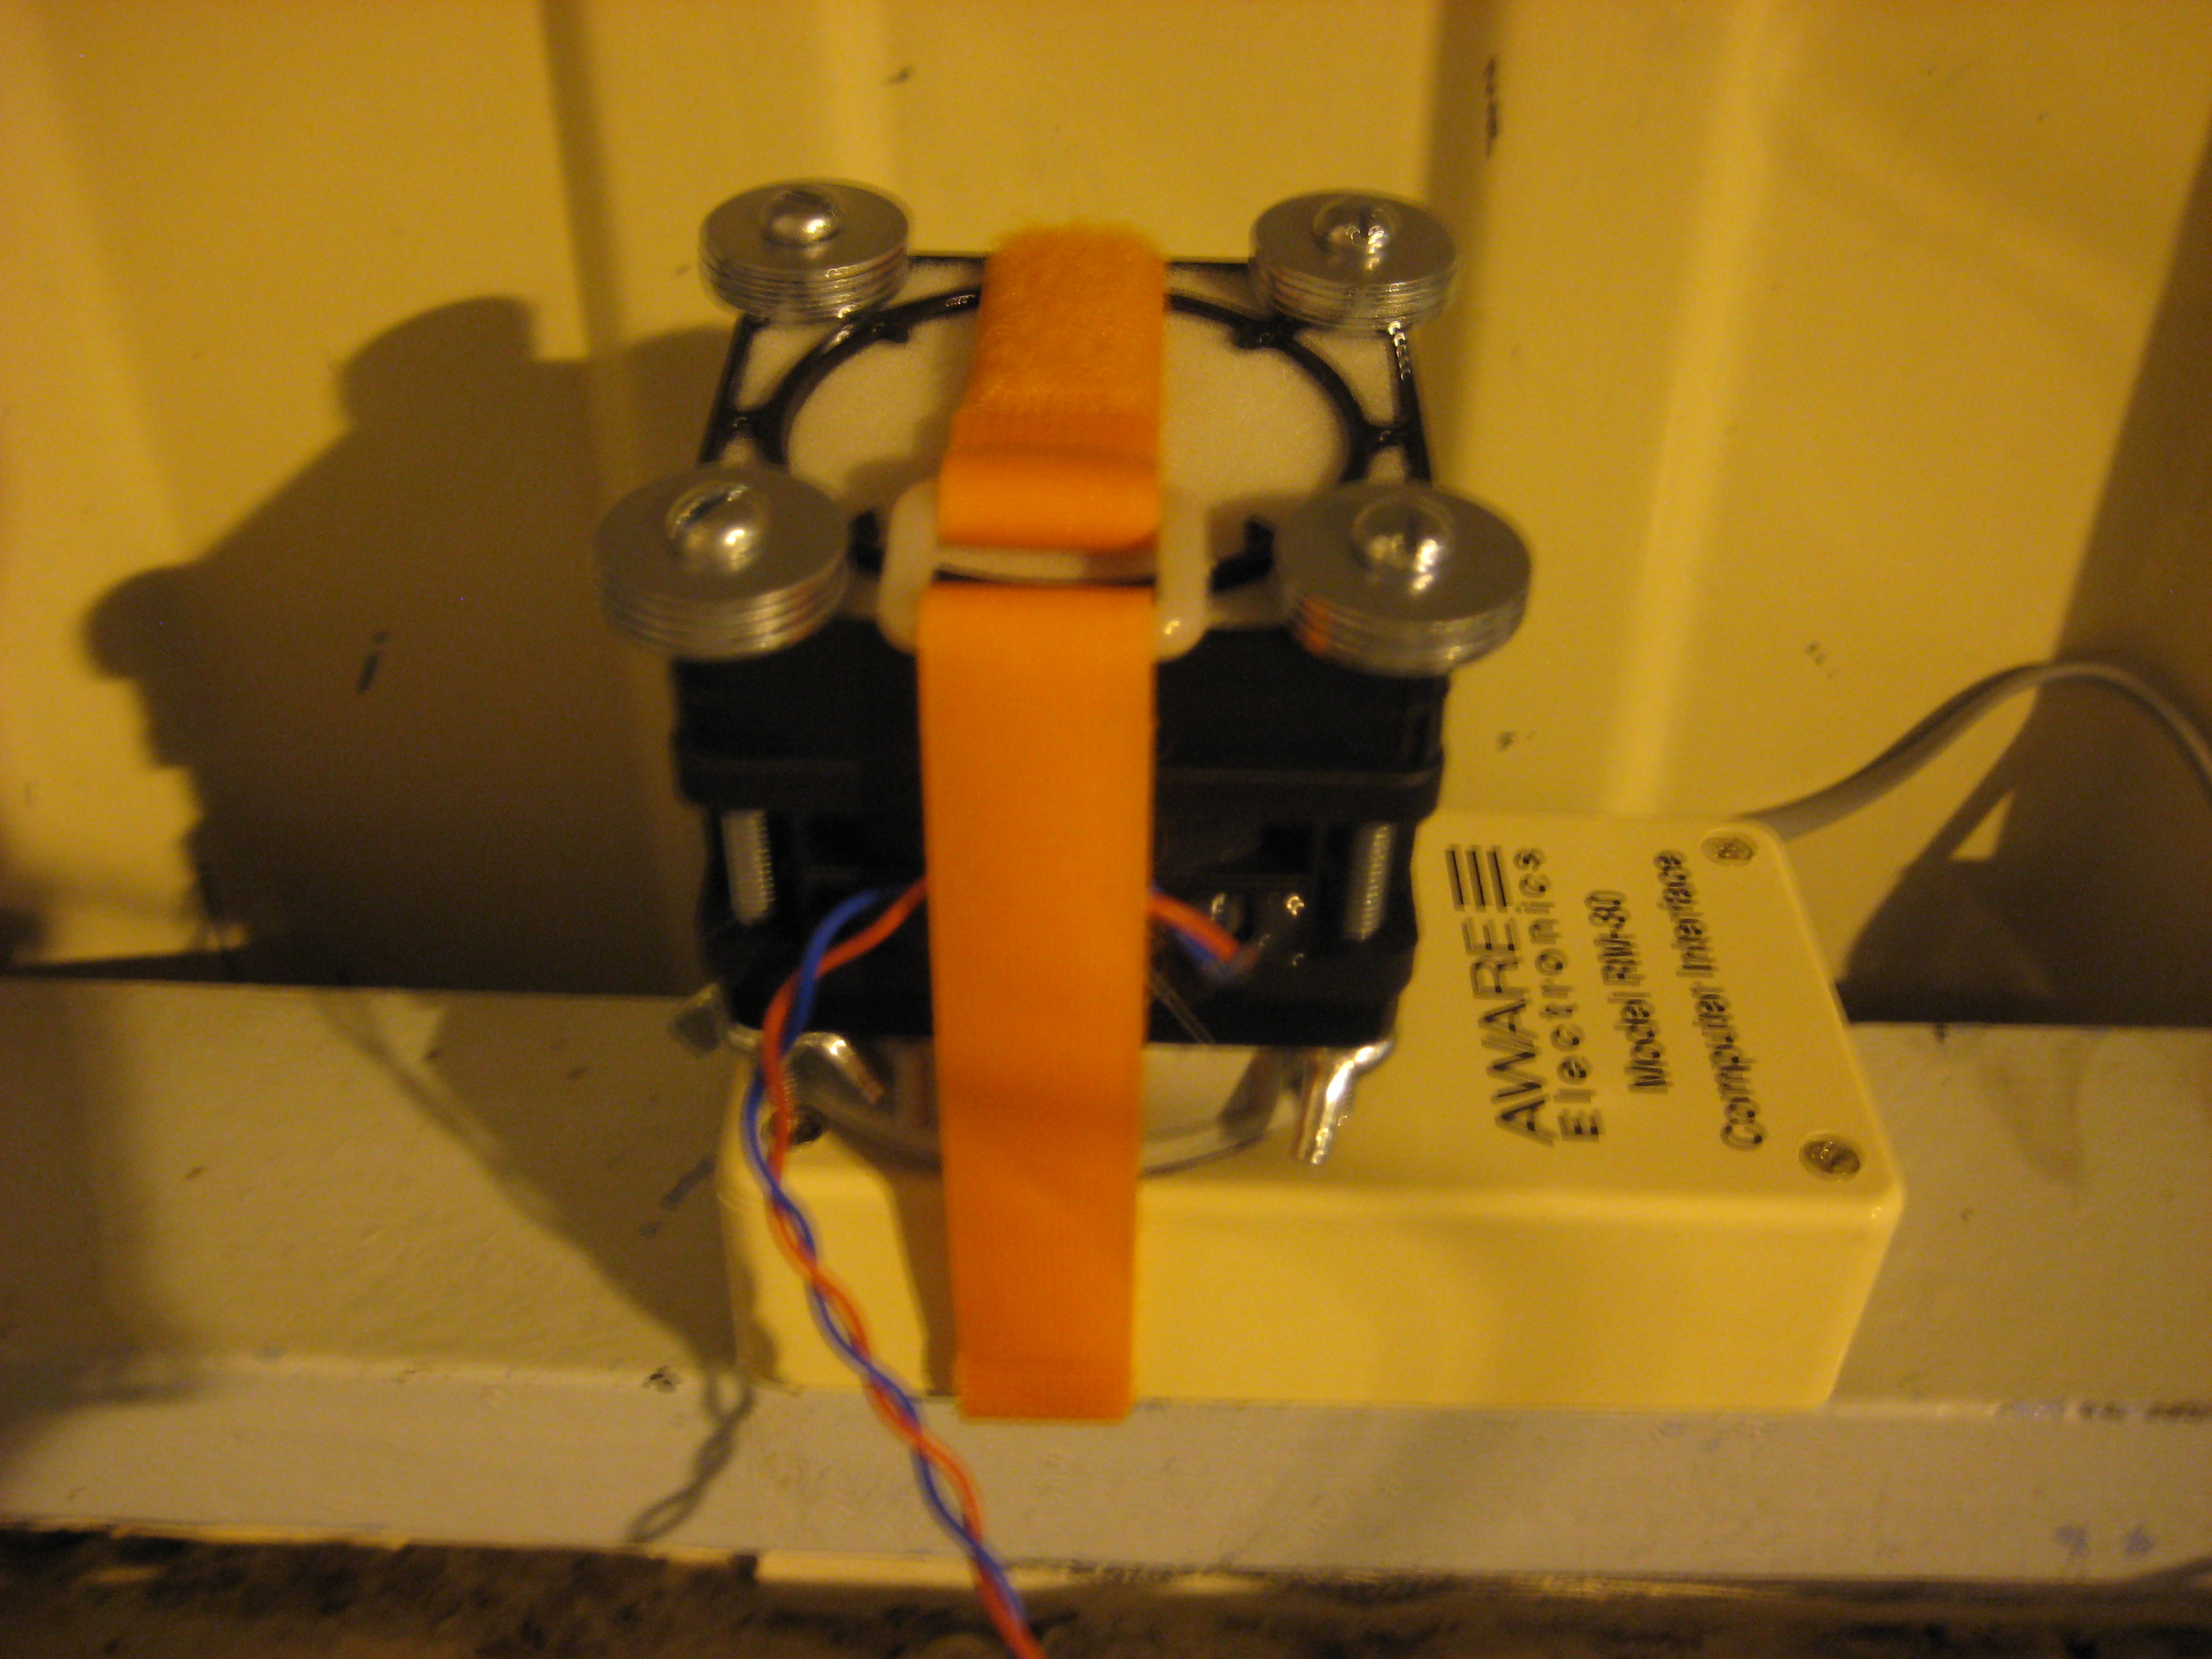
\includegraphics[width=.6\textwidth]{IMG_3817.JPG}
\caption{One of the radon monitors.}
\label{fig16}
\end{figure}

\begin{figure}
\centering
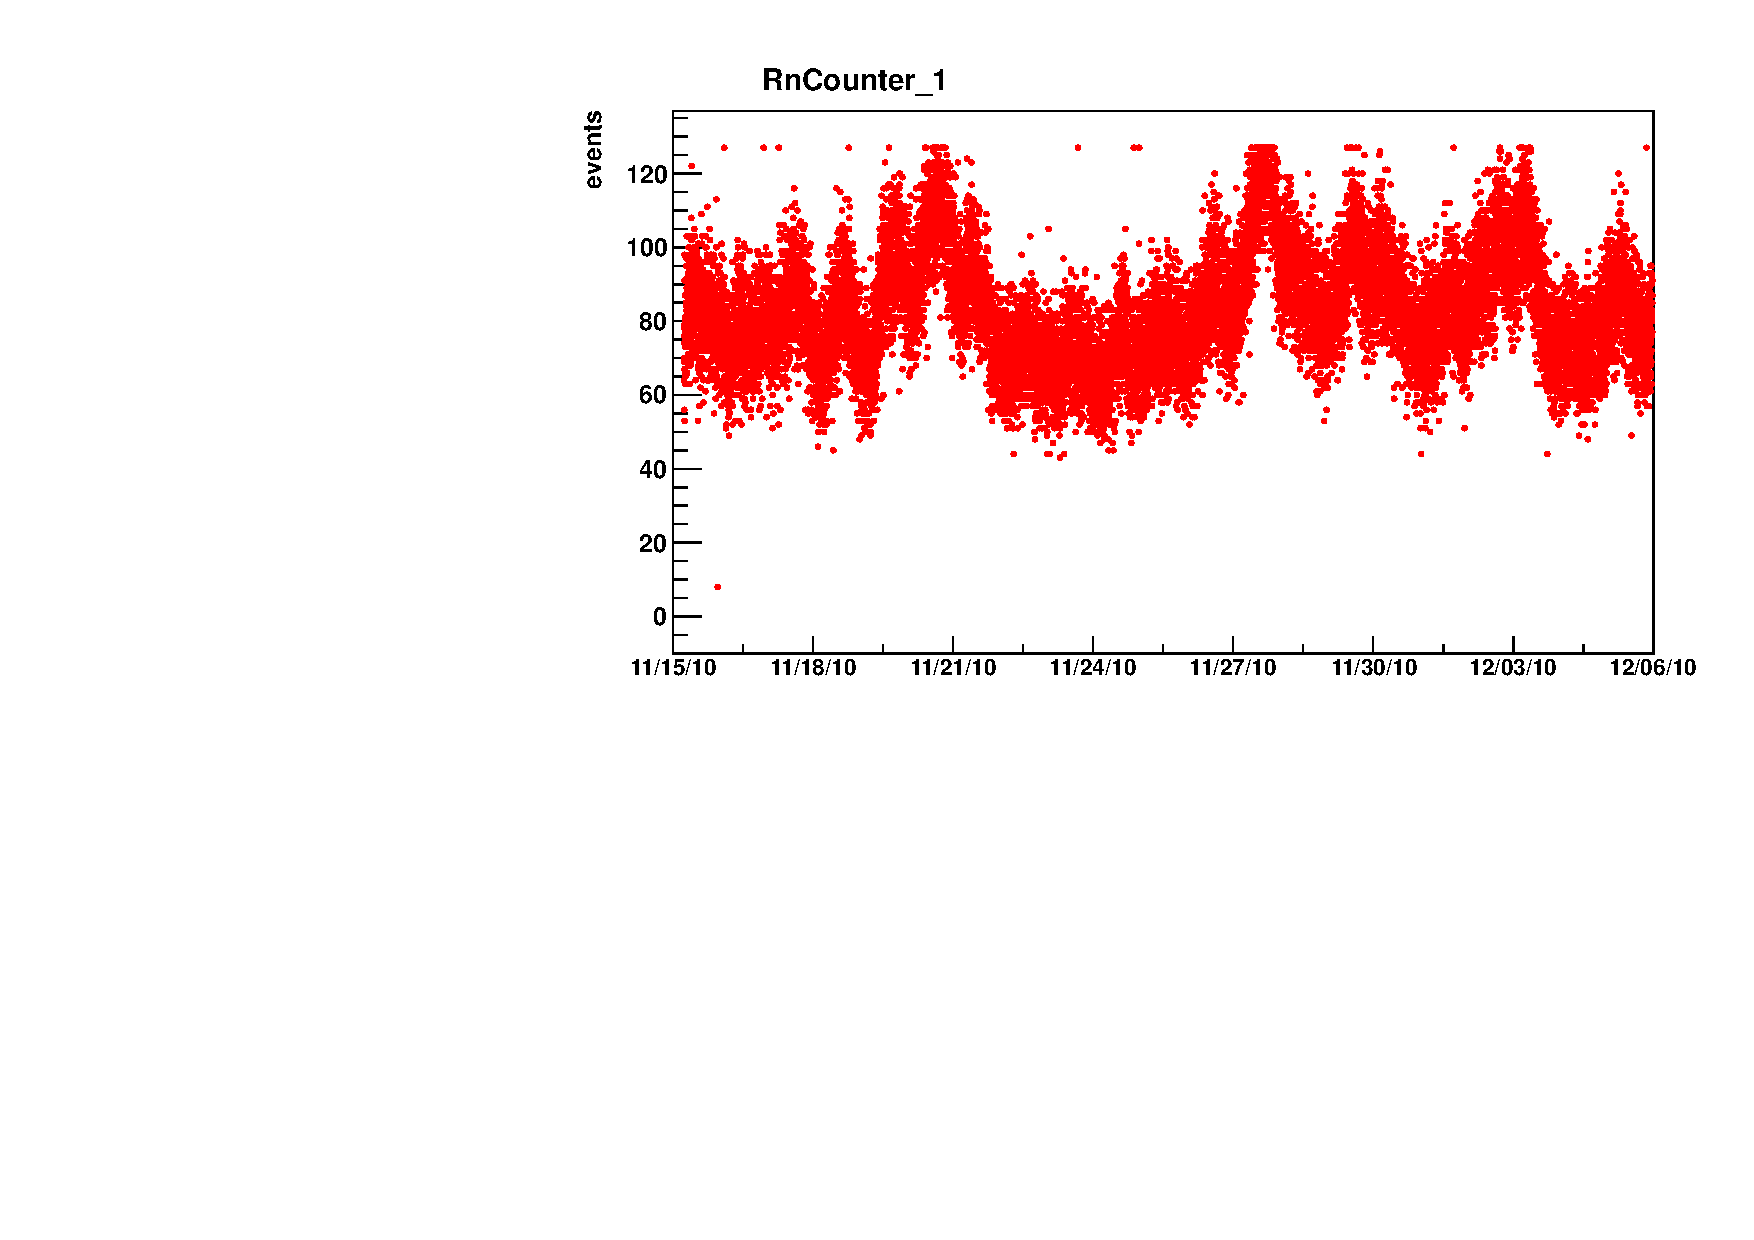
\includegraphics[width=.6\textwidth]{RnCounter01_2010-11-15to2010-12-6.pdf}
\caption{Data from Rn counter from Nov. 2011 to Dec..}
\label{fig17}
\end{figure}
\section{Summary}
Recently high energy experiments require precisely stable environments to control systematic effects. Most of unusual situations in the laboratory can be discover by a physical environment monitoring system before damages happen or to warn shifts immediately. The Double Chooz physical environment monitoring system successfully has reached the goal since 2009 and all historical data can be easily accessed from outside of the laboratory. Because of special requirements from the Double Chooz experiment, this system is low radioactive and waterproof. The low memory and data space requirement is able to running program even in a 10-inch laptop. This system is capable of running in future different varieties of experiments.
\acknowledgments




\begin{thebibliography}{9}

\bibitem{bib1}
Y. Abe et al., \emph{Indication of Reactor $\nu_{e}$ Disappearance in the Double Chooz Experiment}, {\emph{Phys.\ Rev.\ Lett.} {\bf 108} (2012) 131801}.
\bibitem{bib1a}
Y. Abe et al., \emph{Reactor electron antineutrino disappearance in the Double Chooz experiment}, {\emph{Phys.\ Rev.\ D.} {\bf 86} (2012) 052008}.
\bibitem{bib2}
F. Ardellier et al., \emph{Double Chooz, A Search for the Neutrino Mixing Angle theta-13},
\href{http://arxiv.org/abs/hep-ex/0606025}
{\emph{Double Chooz Collaboration} (2006)}
[\astroph{0606025}].
\bibitem{bib3}
T. Konno et al., \emph{Online Data Monitoring Framework Based on Histogram Packaging in Network Distributed Data Acquisition Systems}, {\emph{J.\ Phys.:\ Conf.\ Ser.} {\bf 331} (2011) 022014}.

\bibitem{bib4}
http://www.maxim-ic.com/1-Wire.cfm.
\bibitem{bib5}
Data sheet for DS9490, Dallas Semiconductor, www.maxim-ic.com
\bibitem{bib6}
Data sheet for DS2409, Dallas Semiconductor, www.maxim-ic.com
\bibitem{bib7}
Data sheet for HMC 2003, "Three-Axis Magnetic Sensor Hybrid", Honeywell Solid State Electronics Center.
\bibitem{bib8}
Data sheet for HMC2003, "Magnetic Sensor Hybrid application Circuit", Honeywell Solid State Electronics Center.
\bibitem{bib9}
Data sheet for iButton Devices, Dallas Semiconductor, www.maxim-ic.com
\end{thebibliography}
\end{document}
